\documentclass[letterpaper]{article}
\usepackage[margin=1.0in]{geometry}
\usepackage{authblk}
\usepackage{amsmath, amssymb, amsthm, mathtools}
\usepackage{graphicx}
\usepackage{caption}
\usepackage{subcaption}

\def\btau{\boldsymbol\tau}
\def\bsigma{\boldsymbol\sigma}
\def\bbeta{\boldsymbol\beta}
\def\blambda{\boldsymbol\lambda}

\newcommand{\bs}[1]{\boldsymbol{#1}}
\DeclareMathOperator{\diag}{diag}
\DeclareMathOperator*{\argmin}{\arg\,\min}

\newcommand{\equaldef}{\stackrel{\mathrm{def}}{=}}

\newcommand{\tablab}[1]{\label{tab:#1}}
\newcommand{\tabref}[1]{Table~\ref{tab:#1}}

\newcommand{\theolab}[1]{\label{theo:#1}}
\newcommand{\theoref}[1]{\ref{theo:#1}}
\newcommand{\eqnlab}[1]{\label{eq:#1}}
\newcommand{\eqnref}[1]{\eqref{eq:#1}}
\newcommand{\seclab}[1]{\label{sec:#1}}
\newcommand{\secref}[1]{\ref{sec:#1}}
\newcommand{\lemlab}[1]{\label{lem:#1}}
\newcommand{\lemref}[1]{\ref{lem:#1}}

\newcommand{\mb}[1]{\mathbf{#1}}
\newcommand{\mbb}[1]{\mathbb{#1}}
\newcommand{\mc}[1]{\mathcal{#1}}
\newcommand{\norm}[1]{\left\| #1 \right\|}
\newcommand{\snorm}[1]{\left| #1 \right|}
\newcommand{\LRp}[1]{\left( #1 \right)}
\newcommand{\LRs}[1]{\left[ #1 \right]}
\newcommand{\LRa}[1]{\left\langle #1 \right\rangle}
\newcommand{\LRc}[1]{\left\{ #1 \right\}}
\newcommand{\tanbui}[2]{\textcolor{blue}{\sout{#1}} \textcolor{red}{#2}}
\newcommand{\Grad} {\ensuremath{\nabla}}
\newcommand{\Div} {\ensuremath{\nabla\cdot}}
\newcommand{\Nel} {\ensuremath{{N^\text{el}}}}
\newcommand{\jump}[1] {\ensuremath{\LRs{\![#1]\!}}}
\newcommand{\uh}{\widehat{u}}
\newcommand{\fnh}{\widehat{f}_n}
\renewcommand{\L}{L^2\LRp{\Omega}}
\newcommand{\pO}{\partial\Omega}
\newcommand{\Gh}{\Gamma_h}
\newcommand{\Gm}{\Gamma_{-}}
\newcommand{\Gp}{\Gamma_{+}}
\newcommand{\Go}{\Gamma_0}
\newcommand{\Oh}{\Omega_h}
\newcommand{\ptl}{{\partial}}
\newcommand{\bfsig}{\mbox{\boldmath $\sigma$}}
\newcommand{\bfn}{\mbox{\boldmath $n$}}
\newcommand{\bfH}{\mbox{\boldmath $H$}}
\newcommand{\HdivK}{\bfH(\text{div},K)}
\newcommand{\HOneK}{H^{-1}(K)}
\newcommand{\HOneOmegah}{H^{-1}(\Omega_h)}
\newcommand{\HdivOmegah}{\bfH(\text{div},\Omega_h)}
\newcommand{\vdeltau}{v_{\delta\bs u_h}}
\newcommand{\taudeltau}{\btau_{\delta\bs u_h}}

\newcommand{\eval}[2][\right]{\relax
  \ifx#1\right\relax \left.\fi#2#1\rvert}

\def\etal{{\it et al.~}}

\newcommand{\vect}[1]{\ensuremath\boldsymbol{#1}}
\newcommand{\tensor}[1]{\underline{\vect{#1}}}
\newcommand{\del}{\Delta}
\newcommand{\grad}{\nabla}
\newcommand{\curl}{\grad \times}
\renewcommand{\div}{\grad \cdot}
\newcommand{\ip}[1]{\left\langle #1 \right\rangle}
\newcommand{\eip}[1]{a\left( #1 \right)}
\newcommand{\pd}[2]{\frac{\partial#1}{\partial#2}}
\newcommand{\pdd}[2]{\frac{\partial^2#1}{\partial#2^2}}

\newcommand{\circone}{\ding{192}}
\newcommand{\circtwo}{\ding{193}}
\newcommand{\circthree}{\ding{194}}
\newcommand{\circfour}{\ding{195}}
\newcommand{\circfive}{\ding{196}}

\def\arr#1#2#3#4{\left[
\begin{array}{cc}
#1 & #2\\
#3 & #4\\
\end{array}
\right]}
\def\vecttwo#1#2{\left[
\begin{array}{c}
#1\\
#2\\
\end{array}
\right]}
\def\vectthree#1#2#3{\left[
\begin{array}{c}
#1\\
#2\\
#3\\
\end{array}
\right]}
\def\vectfour#1#2#3#4{\left[
\begin{array}{c}
#1\\
#2\\
#3\\
#4\\
\end{array}
\right]}

\renewcommand{\arraystretch}{2.0}

\newtheorem{proposition}{Proposition}
\newtheorem{corollary}{Corollary}
\newtheorem{theorem}{Theorem}
\newtheorem{lemma}{Lemma}

\newcommand{\G} {\Gamma}
\newcommand{\Gin} {\Gamma_{in}}
\newcommand{\Gout} {\Gamma_{out}}

\title{Locally Conservative Discontinuous Petrov-Galerkin Finite Elements for
Fluid Problems}
\author{Truman Ellis} 
\author{Leszek Demkowicz}
\author{Jesse Chan}
\affil{Institute for Computational Engineering and Sciences,\\
The University of Texas at Austin, \\
Austin, TX 78712}
\date{}

\begin{document}
\maketitle

\begin{abstract}
\end{abstract}

\section{Intoduction}
The discontinuous Petrov-Galerkin (DPG) method with optimal test functions has
been under active development for convection-diffusion type systems
\cite{DPG1, DPG2, DPG3, DPG5, DemkowiczHeuer, ChanHeuerThanhDemkowicz2012,
MoroNguyenPeraire11}. In this paper, we develop a theory for the locally conservative
formulation of DPG for convection-diffusion type equations and supplement this
with extensive numerical results.

\subsection{Importance of Local Conservation}
Locally conservative methods hold a special place for numerical analysts in
the field of fluid dynamics. 
Perot\cite{Perot2011} argues
\begin{quote}
Accuracy, stability, and consistency are the mathematical concepts that are
typically used to analyze numerical methods for partial differential equations
(PDEs). These important tools quantify how well the mathematics of a PDE is
represented, but they fail to say anything about how well the physics of the
system is represented by a particular numerical method. In practice, physical
fidelity of a numerical solution can be just as important (perhaps even more
important to a physicist) as these more traditional mathematical concepts. A
numerical solution that violates the underlying physics (destroying mass or
entropy, for example) is in many respects just as flawed as an unstable
solution.
\end{quote}

The discontinuous Petrov-Galerkin finite element method has been described as
least squares finite elements with a twist. The key difference is that least
square methods seek to minimize the residual of the solution in the $L^2$
norm, while DPG seeks the minimization in a dual norm realized through the
inverse Riesz map. Exact mass conservation has been an issue that has plagued
least squares finite elements for a long time. Several approaches have been
used to try to adress this. Chang and Nelson\cite{ChangNelson1997} developed
the \emph{restricted LSFEM}\cite{ChangNelson1997} by augmenting the least squares
equations with a Lagrange multiplier explicitly enforcing mass conservation
element-wise. Our conservative formulation of DPG takes a similar approach and
both methods share similar negative of transforming a minimization method to a
saddle-point problem.

\subsection{DPG is a Minimum Residual Method}
Roberts \etal presents a brief history and derivation of DPG with optimal test functions in
\cite{DPGStokes}. We follow his derivation of the standard DPG method as a
minumum residual method. Let $U$ be the trial Hilbert space and $V$ the test
Hilbert space for a well-posed variational problem $b(u,v)=l(v)$. In operator
form this is $Bu=l$, where $B:U\rightarrow V'$. We seek to minimize the
residual for the discrete space $U_h\subset U$:
\begin{equation}
u_h=\argmin_{u_h\in U_h}\frac{1}{2}\norm{Bu_h-l}^2_{V'}\,.
\label{minresidual}
\end{equation}
Recalling that the Riesz operator $R_V:V\rightarrow V'$ is an isometry defined
by
\[
\LRa{R_Vv,\delta v}=\LRp{v,\delta v}_V,\quad\forall\delta v\in V,
\]
we can use the Riesz inverse to minimize in the $V$-norm rather than its dual:
\begin{equation}
\frac{1}{2}\norm{Bu_h-l}^2_{V'}=\frac{1}{2}\norm{R_V^{-1}(Bu_h-l)}^2_V
=\frac{1}{2}\LRp{R_V^{-1}(Bu_h-l),R_V^{-1}(Bu_h-l)}_V\,.
\label{eq:rieszapplied}
\end{equation}
The first order optimality condition for \eqnref{rieszapplied} requires
the G\^ateaux derivative to be zero in all directions $\delta u \in
U_h$, i.e.,
\[
\left(R_V^{-1}(Bu_h-l),R_V^{-1}B\delta u\right)_V = 0, \quad \forall \delta u \in U. 
\]
By definition of the Riesz operator, this is equivalent to
\begin{equation}
\LRa{Bu_h-l,R_V^{-1}B\delta u_h}=0\quad\forall\delta u_h\in U_h\,.
\label{eq:DPGbilinearform}
\end{equation}
Now, we can identify $v_{\delta u_h}\coloneqq R_V^{-1}B\delta u_h$ as the
optimal test function for trial function $\delta u_h$. Define $T:=R_V^{-1}B:U_h\rightarrow V$ as the trial-to-test operator. Now we can rewrite
\eqnref{DPGbilinearform} as
\begin{equation}
b(u_h,v_{\delta u_h})=l(v_{\delta u_h}).
\label{eq:DPGmethod}
\end{equation}
The DPG method then is to solve \eqnref{DPGmethod} with optimal test functions
$v_{\delta u_h}\in V$ that solve the auxiliary problem
\begin{equation}
\LRp{v_{\delta u_h},\delta v}_V=\LRa{R_Vv_{\delta u_h},\delta v}
=\LRa{B\delta u_h,\delta v}=b(\delta u_h,\delta v)\,,\quad\forall\delta v\in V.
\label{eq:optimaltestproblem}
\end{equation}
Using a continuous test basis would result in a global solve for every optimal
test function. Therefore DPG uses a discontinuous test basis which makes each
solve element-local and much more computationally tractable. Of course,
\eqnref{optimaltestproblem} still requires the inversion of the
infinite-dimensional Riesz map, but approximating $V$ by a finite
dimensional $V_h$ which is of a higher polynomial degree than $U_h$ (hence
``enriched space'') works well in practice.

No assumptions have been made so far on the definition of the inner product on
$V$. In fact, proper choice of $\LRp{\cdot,\cdot}_V$ can make the difference
between a solid DPG method and one that suffers from robustness issues.

\section{Analysis}
We now proceed to develop a locally conservative formulation of DPG for
convection-diffusion type problems, but there are a few terms that we need to
define first. If $\Omega$ is our problem domain, then we can partition it into
finite elements $K$ such that
\[
\overline{\Omega} = \bigcup_K  \bar{K},\: \quad K \text { open},
\]
with corresponding {\em skeleton} $\Gamma_h$ and {\em interior
  skeleton} $\Gamma_h^0$,
\[
\Gamma_h := \bigcup_K \partial K\qquad \Gamma_h^0 := \Gamma_h - \Gamma.
\]
We define broken Sobolev spaces element-wise:
\[
\begin{array}{rl}
H^1(\Omega_h) & := \prod_K H^1(K), \\[8pt]
\bfH(\text{div},\Omega_h) & := \prod_K \bfH(\text{div},K).
\end{array}
\]
We also need the trace spaces:
\[
\begin{array}{rl}
H^\frac{1}{2}(\Gamma_h) & := \left\{ \hat{v} = \{\hat{v}_K \} \in \prod_K H^{1/2}(\ptl K) \: :
\: \exists v \in H^1(\Omega) : v\vert_{\ptl K} = \hat{v}_K \right\}, \\[8pt]
H^{-\frac{1}{2}}(\Gamma_h) & := \left\{ {\hat{\sigma}}_n = \{ {\hat{\sigma}}_{Kn} \}\in \prod_K H^{-1/2}(\ptl K) \: : \: \exists \bfsig \in \bfH(\text{div},\Omega)
: {\hat{\sigma}}_{Kn} = (\bfsig \cdot \bfn)\vert_{\ptl K} \right\},
\end{array}
\]
which are developed more precisely in \cite{DPGStokes}.

\subsection{Element Conservative Convection-Diffusion}
Now that we have briefly outlined the abstract DPG method, let us apply it to
the convection-diffusion equation. The strong form of the steady
convection-diffusion problem with homogeneous Dirichlet boundary conditions reads
\[
\left\{
\begin{array}[c]{rrl}
\div(\bs\beta u)-\epsilon\del u & =f & \text{in }\Omega\\
u & =0 & \text{on }\Gamma\,,
\end{array}
\right.
\]
where $u$ is the property of interest, $\bs\beta$ is the convection vector,
and $f$ is the source term. Nonhomogeneous Dirichlet and Neumann boundary
conditions are straightforward but would add technicality to the following
discussion. Let us write this as an equivalent system of first
order equations:
\begin{align*}
\div(\bs\beta u-\bs\sigma)&=f\\
\frac{1}{\epsilon}\bs\sigma-\grad u&=\bs0\,.
\end{align*}
If we then multiply the top equation by some scalar test function $v$ and the
bottom equation by some vector-valued test function $\tau$, we can integrate by
parts over each element $K$:
\begin{equation}
\label{eq:preultraweak}
\begin{aligned}
-(\bbeta u-\bsigma,\nabla v)_K+((\bbeta
u-\bsigma)\cdot\mathbf{n},v)_{\partial K}&=(f,v)_K\\
\frac{1}{\epsilon}(\bsigma,\btau)_K+(u,\nabla\cdot\btau)_K
-(u,\tau_n)_{\partial K}&=0\,.
\end{aligned}
\end{equation}
The discontinuous Petrov-Galerkin method refers to the fact that we are using
discontinuous optimal test functions that come from a space differing from the
trial space. It does not specify our choice of trial space. Nevertheless, many
considerations of DPG in the literature \cite{} associate DPG with the
so-called ``ultra-weak formulation.'' We will follow the same derivation for
the convection-diffusion equation, but we emphasize that other formulations
are available. Thus, we seek field variables $u\in L^2(K)$ and
$\bsigma\in\mb{L^2}(K)$. Mathematically, this leaves their traces on element
boundaries undefined, and in a manner similar to the hybridized discontinuous
Galerkin method, we define new unknowns for trace $\hat u$ and flux $\hat t$.
Applying these definitions to \eqnref{preultraweak} and adding the two
equations together, we arrive at our desired variational problem. 

Find
$\bs u:=(u,\bsigma,\hat u,\hat t)
\in\bs U:=L^2(\Omega_h)\times \bs L^2(\Omega_h)\times H^{1/2}(\Gamma_h)\times H^{-1/2}(\Gamma_h)$ 
such that
\begin{align}
\label{eq:variationalFormulation}
\underbrace{-(\bbeta u-\bsigma,\nabla v)_K+(\hat t,v)_{\partial K}
+ \frac{1}{\epsilon}(\bsigma,\btau)_K
+(u,\nabla\cdot\btau)_K
-(\hat u,\tau_n)_{\partial K}}_{b(\mathbf{u}, \mathbf{v})}
&=\underbrace{\:(f,v)_K\genfrac{}{}{0pt}{}{}{}}_{l(\mathbf{v})} &\text{in }\Omega \\
u&=0 &\text{on }\Gamma\\
\end{align}
for all $\bs v:=(v,\btau)\in
\bs V:=H^1(\Omega_h)\times\bfH(\text{div},\Omega_h)$.

Let $\bs U_h:=U_h\times\bs S_h\times\hat U_h\times\hat F_h\subset L^2(\Omega_h)\times\bs
L^2(\Omega_h)\times H^{\frac{1}{2}}(\Gamma_h)\times H^{-\frac{1}{2}}(\Gamma_h)$
be a finite-dimensional subspace, and let $\bs u_h:=(u_h.\bsigma_h,\hat
u_h\hat t_h)\in\bs U_h$ be a group variable. The element conservative DPG scheme is
derived from the Lagrangian:
\begin{equation}
L(\bs u_h,\lambda_k)=\frac{1}{2}\norm{R_V^{-1}(b(\bs
u_h,\cdot)-(f,\cdot))}^2_{\bs V}-\sum_K\lambda_K(b(\bs u_h,(1_K,\bs0))-l((1_K,\bs0)))\,,
\label{eq:lagrangian}
\end{equation}
where $(1_K,\bs0)$ is the test function in which $v=1$ on element $K$ and 0 elsewhere and $\btau=\bs0$ everywhere.

Taking the G\^ateaux derivatives as before, we arrive at the following system
of equations:
\begin{equation}
\left\{
\begin{array}[c]{rll}
b(\bs u_h,T(\delta\bs u_h))-\sum_K\lambda_K b(\bs u_h,(1_K,\bs0))
&=(f,T(\delta\bs u_h)) & \forall\delta\bs u_h\in\bs U_h\\
b(\bs u_h,(1_K,\bs0)) &=(f,(1_K,\bs0)) & \forall K\,,
\end{array}
\right.
\label{eq:conservativeSystem}
\end{equation}
where $T:=R_V^{-1}B:\bs U_h\rightarrow\bs V$ is the same trial-to-test operator as in the original formulation.

Since the trial-to-test operator selectively produces test functions in
$H^1(\Omega_h)$ and $\bs H(\text{div},\Omega_h)$, denote the result
$v_{\delta\bs u_h}$ when $T(\delta u_h)\in H^1(\Omega_h)$ and
$\btau_{\delta\bs u_h}$ when $T(\delta u_h)\in \bs H(\text{div},\Omega_h)$.
Then, putting \eqref{eq:conservativeSystem} into more concrete terms for
convection-diffusion, we get:
\begin{equation}
\left\{
\begin{array}[c]{rll}
-(\bbeta u-\bsigma,\nabla \vdeltau)+\langle\hat t,\vdeltau\rangle
+ \frac{1}{\epsilon}(\bsigma,\taudeltau)
+(u,\nabla\cdot\taudeltau)
-\langle\hat u,\taudeltau\cdot\bs n\rangle\\
-\sum_K\lambda_K (\delta\hat t,(1_K,\bs0))
&=(f,\vdeltau) & \forall\delta\bs u_h\in\bs U_h\\
\langle\hat t,(1_K,\bs0)\rangle &=(f,(1_K,\bs0)) & \forall K\,.
\end{array}
\right.
\label{eq:conservativeConfusionSystem}
\end{equation}

The optimal test functions are determined by solving local problems determined
by the choice of test norm. For illustrative purposes we choose the robust
test norm developed by Chan \etal\cite{ChanHeuerThanhDemkowicz2012}. With this
choice, we get our local problem:

Find $\vdeltau\in\HOneK,\,\taudeltau\in\HdivK$ such that:
\begin{align}
(\nabla\cdot\taudeltau,&\nabla\cdot\delta\btau)_K
+\min\left\{\frac{1}{\epsilon},\frac{1}{|K|}\right\}(\taudeltau,\delta\btau)_K
+\epsilon(\nabla\vdeltau,\nabla \delta v)_K
+(\bbeta\cdot\nabla\vdeltau,\bbeta\cdot\nabla \delta v)_K\nonumber\\
&+\alpha\min\left\{\sqrt{\frac{\epsilon}{|K|}},1\right\}(\vdeltau,\delta v)_K
=b(\delta\bs u_h,(\delta v,\delta\btau))
\quad\quad\forall\delta v\in\HOneK,\,\delta\btau\in\HdivK\,,
\label{eq:localSolve}
\end{align}
where, typically, $\alpha=1$.

We can decompose the discrete flux space $\hat F_h$ into element conserving
fluxes and some algebraic complement:
\begin{equation}
\hat F_h=\hat F_h^c\oplus\hat F_h^{nc}\,,\quad\hat 
F_h^{c}:=\{\hat t:\langle\hat t,(1_K,\bs0)\rangle=0\quad\forall K\}\,.
\label{eq:decomposition}
\end{equation}
This may be accomplished by employing for fluxes in $\hat F_h^{c}$ traces of
curls, $\nabla\times\phi$. 

In practice, we solve \eqref{eq:conservativeConfusionSystem} as a fully 
coupled system of equations, but for didactic purposes, we can examine it 
one piece at a time. If we restrict \eqref{eq:conservativeConfusionSystem}$_1$
to $\delta\hat t\in\hat F_h^{nc}$, the Lagrange multiplier term drops out and we 
left with a system that we can solve for $u_h$, $\bsigma_h$, $\hat u_h$, and 
$\hat t_h^c\in\hat F^c_h$.

Restricting ourselves to $\delta\hat t\in\hat
F_h^{c}$ in \eqref{eq:conservativeConfusionSystem}$_1$, we obtain a system  of
equations that can be solved for $u_h$, $\bsigma_h$, $\hat u$, and $\hat
t\in\hat F_h^c$. The remaining fluxes, $\hat t\in\hat F_h^{nc}$ are determined
from \eqref{eq:conservativeConfusionSystem}$_2$. Finally, testing with $\hat
t\in\hat F_h^{nc}$ in \eqref{eq:conservativeConfusionSystem}$_1$, we obtain a
system of equations that can be solved for Lagrange multipliers $\lambda_K$.

Additionally, we can pass in local problem \eqref{eq:localSolve} with
$\alpha\rightarrow0$. The fact that the test functions will be determined then
up to a constant does not matter, for $\delta\hat t\in\hat F_h^c$, equation
\eqref{eq:conservativeConfusionSystem}$_1$ is orthogonal to constants. 
Mathematically, we are dealing with equivalence classes of functions, but in order 
to obtain a single function that we can deal with numerically, we replace the alpha 
term with a zero mean scaling condition to obtain the new test norm,
\begin{align}
(\nabla\cdot\taudeltau,&\nabla\cdot\delta\btau)_K
+\min\left\{\frac{1}{\epsilon},\frac{1}{|K|}\right\}(\taudeltau,\delta\btau)_K
\nonumber\\
&+\epsilon(\nabla\vdeltau,\nabla \delta v)_K
+(\bbeta\cdot\nabla\vdeltau,\bbeta\cdot\nabla \delta v)_K
+\frac{1}{|K|^2}\int_K\vdeltau\delta v\,,
\label{eq:localSolveMod}
\end{align}
where the $\frac{1}{|K|^2}$ coefficient is needed to make the zero mean term 
scale correctly with $h$. Numerically this helps a good deal with the condition
numbers of the local solve.

It is convenient to be able to take $\alpha\rightarrow0$ as we will see in
some later numerical experiments.

\subsection{Proof of Convergence}
We cannot directly use Brezzi's theorem, but we can reproduce his argument.
First of all, variational formulation \eqref{eq:variationalFormulation} is
equivalent to:

Find $\bs u\in\bs U$ such that
\begin{equation}
b(\bs u,T(\delta\bs u))=(f,T(\delta\bs u))\quad\forall\bs v\in\bs V\,.
\label{eq:bilinearForm}
\end{equation}
This is because the trial-to-test operator $T=R_V^{-1}B$ is an isomorphism.

Restricting ourselves to $\delta\hat t_h\in\hat F_h^c$, and subtracting
\eqref{eq:bilinearForm} from \eqref{eq:conservativeConfusionSystem}, we have
the Galerkin orthogonality condition:
\begin{align}
\label{eq:galerkinOrthogonality}
\frac{1}{\epsilon}(\bsigma_h-\bsigma,\taudeltau)
&+(u_h-u,\nabla\cdot\taudeltau)
-\langle\hat u_h-\hat u,\taudeltau\cdot\bs n\rangle
\nonumber\\
&-(\bbeta(u_h-u)-(\bsigma_h-\bsigma),\nabla\vdeltau)
+\langle\hat t_h-\hat t,\vdeltau\rangle
\\
&\hspace{25ex}\forall(\delta u_h,\delta\bsigma_h,\delta\hat u_h,\delta\hat t_h)
\in U_h\times\bs S_h\times\hat U_h\times\hat F_h^c\,.
\nonumber
\end{align}

We begin with an equivalent of Brezzi's \emph{discrete inf-sup in kernel
condition}.
\begin{lemma}
\label{lemma:infsuplemma}
The following condition holds:
\begin{align}
\sup_{\stackrel{
(\delta u_h,\delta\bsigma_h,\delta\hat u,\delta\hat t)\in}
{U_h\times\bs S_h\times\hat U_h\times\hat F_h^c}
}
\frac{\snorm{
b((u_h,\bsigma_h,\hat u_h,\hat t_h), (\vdeltau,\taudeltau))
% \frac{1}{\epsilon}(\bsigma_h,\taudeltau)
% +(u_h,\nabla \cdot\taudeltau)
% -\langle\hat u_h,\taudeltau\cdot\bs n\rangle
% -(\bbeta u_h-\bsigma_h,\nabla\vdeltau)
% +\langle\hat t_h,\vdeltau\rangle
}}
{\norm{(\vdeltau,\taudeltau)}}
\ge\alpha\norm{(u_h,\bsigma_h,\hat u_h,\hat t_h)}\quad\nonumber\\
\forall(u_h,\bsigma_h,\hat u_h,\hat t_h)
\in U_h\times\bs S_h\times\hat U_h\times\hat F_h^c\,.
\label{eq:infsup}
\end{align}

\end{lemma}
\begin{proof}
By the very construction of the trial-to-test operator, the supremum on the
left is equal to
\begin{equation}
\norm{T(u_h,\bsigma_h,\hat u_h,\hat t_h)}_{V}
=\norm{R_V^{-1}B(u_h,\bsigma_h,\hat u_h, \hat t_h)}_{V}
=\norm{B(u_h,\bsigma_h,\hat u_h, \hat t_h)}_{V'}
\label{eq:infsupproof}
\end{equation}
The condition follows now from the fact that operator $B$ is bounded below,
i.e. bilinear form \linebreak$b((u_h,\bsigma_h,\hat u_h, \hat t_h),(v,\btau))$ satisfies
the inf-sup condition.
\end{proof}

Assume additionally that flux decomposition \eqref{eq:decomposition} is
orthogonal. We begin by decomposing $\hat t_h$,
\begin{equation}
\hat t_h=\hat t_h^{c}+\hat t_h^{nc}\,.
\label{eq:fluxdecomposition}
\end{equation}
Next, we use the triangle inequality,
\begin{align}
\label{eq:triangle}
\norm{(u-u_h,\bsigma-\bsigma_h,\hat u-\hat u_h, \hat t-\hat t_h)}&=
\norm{(u-u_h,\bsigma-\bsigma_h,\hat u-\hat u_h, \hat t-(\hat t_h^c+\hat t_h^{nc}))}\nonumber\\
&\le\norm{(u-w_h,\bsigma-\bs s_h,\hat u-\hat w_h, \hat t-(\hat r_h^c+\hat t_h^{nc}))}\\
&\hspace{3ex}+\norm{(w_h-u_h,\bs s_h-\bsigma_h,\hat w_h-\hat u_h, \hat r_h^c-\hat t_h^c)}\nonumber
\end{align}
where $w_h\in U_h$, $\bs s_h\in\bs S_h$, $\hat w_h\in\hat U_h$, and $\hat
r_h^{c}\in\hat F_h$ are arbitrary. The inf-sup in kernel condition now
implies:
\begin{align}
\label{eq:estimate}
&\norm{(w_h-u_h,\bs s_h-\bsigma_h,\hat w_h-\hat u_h, \hat r_h^c-\hat t_h^c)}\\
&\hspace{8ex}\le\frac{1}{\alpha}
\sup_{\stackrel{
(\delta u_h,\delta\bsigma_h,\delta\hat u,\delta\hat t)\in}
{U_h\times\bs S_h\times\hat U_h\times\hat F_h^c}
}
\frac{\snorm{
b( (w_h-u_h,\bs s_h-\bsigma_h,\hat w_h-\hat u_h,\hat r_h^c-\hat t_h^c),
(\vdeltau,\taudeltau))
}}
{\norm{(\vdeltau,\taudeltau)}}\nonumber\\
&\hspace{8ex}\le\frac{1}{\alpha}
\sup_{\stackrel{
(\delta u_h,\delta\bsigma_h,\delta\hat u,\delta\hat t)\in}
{U_h\times\bs S_h\times\hat U_h\times\hat F_h^c}
}
\frac{\snorm{
b( (w_h-u_h,\bs s_h-\bsigma_h,\hat w_h-\hat u_h,\hat r_h^c+\hat t_h^{nc}-\hat t),
(\vdeltau,\taudeltau))
}}
{\norm{(\vdeltau,\taudeltau)}}\nonumber\\
&\hspace{8ex}\le\frac{1}{\alpha}
\norm{(w_h-u_h,\bs s_h-\bsigma_h,\hat w_h-\hat u_h,\hat t-(\hat r_h^c+\hat
t_h^{nc}))}
\end{align}
% \frac{1}{\epsilon}(\bs s_h-\bsigma_h,\taudeltau)
% +(w_h-u_h,\nabla \cdot\taudeltau)
% -\langle\hat w_h-\hat u_h,\taudeltau\cdot\bs n\rangle
% -(\bbeta (w_h-u_h)-(\bs s_h-\bsigma_h),\nabla\vdeltau)
% +\langle\hat r_h^c-\hat t_h^c,\vdeltau\rangle
where the second step follows from the Galerkin orthogonality condition
\eqref{eq:galerkinOrthogonality}, and the last step is a consequence of the
minimum energy extension norm for fluxes. Cobining with \eqref{eq:triangle},
we get the final stability result:
\begin{equation}
\norm{(u-u_h,\bsigma-\bsigma_h,\hat u-\hat u_h,\hat t-\hat t_h)}
\leq\left(1+\frac{1}{\alpha}\right)
\inf_{\stackrel{
(w_h,\bs s_h,\hat w,\hat r_h^c)\in}
{U_h\times\bs S_h\times\hat U_h\times\hat F_h^c}
}
\norm{(u-w_h,\bsigma-\bs s_h,\hat u-\hat w,\hat t-(\hat r_h^c+\hat t_h^{nc}))}
\,.
\label{eq:stability}
\end{equation}

\section{Numerical Experiments}
We explore each of the following experiments with two sets of test norms: the
standard graph norm, and the aforementioned robust norm.

\subsection{Erickson-Johnson Model Problem}
The Erickson-Johnson problem is one of the few convection-diffusion problems
with a known analytical solution. Take a domain $\Omega=[0,1]^2$, with
$\bbeta=(1,0)^T$, $f=0$ and boundary conditions $\hat t=u_0$ when
$\beta_n\le0$, and $u_0$ is the trace of the exact solution. For
$n=1,2,\cdots$, let
$\lambda_n=n^2*\pi^2*\epsilon$,
$r_n=\frac{1+\sqrt{1+4\epsilon\lambda_n}}{2\epsilon}$, and 
$s_n=\frac{1-\sqrt{1+4\epsilon\lambda_n}}{2\epsilon}$, the exact solution
is
\begin{equation}
u(x,y)=C_0+\sum_{n=1}^\infty C_n\frac{\exp(s_n(x-1))-\exp(r_n(x-1))}
{r_n\exp(-s_n)-s_n\exp(-s_n)}\cos(n\pi y)\,.
\label{eq:ericksonExact}
\end{equation}
Taking $\epsilon=0.01$, $C_1=1$, and $C_{n\neq1}=0$, the exact solution looks
like Figure \ref{fig:erickson}. We solve this problem with both conservative
and nonconservative formulations of DPG with both graph and robust test norms.

\begin{figure}[h!]
\centering
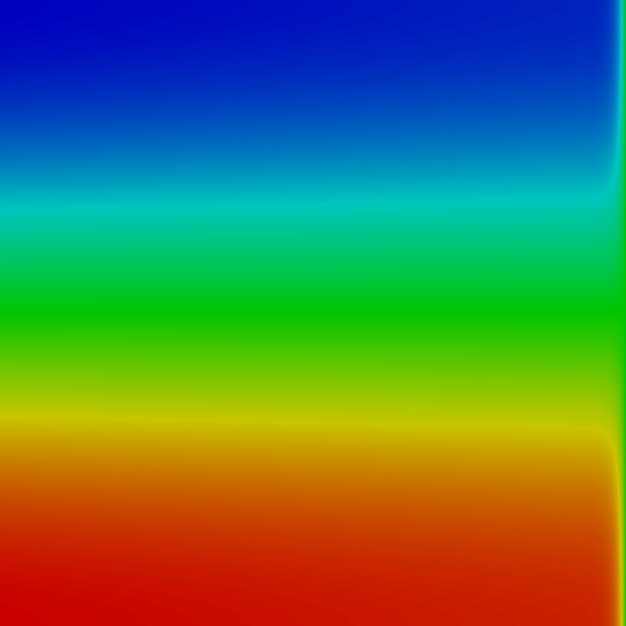
\includegraphics[width=0.6\textwidth]{figs/Erickson/exact.png}
\caption{Erickson-Johnson exact solution}
\label{fig:erickson}
\end{figure}

We plot the $L^2$ and energy error for the various methods in Figures
\ref{fig:ericksonGraphError} and \ref{fig:ericksonRobustError}. Encouragingly,
the conservative and nonconservative plots appear to lay right on top of each
other. This indicates that the conservative formulation at least doensn't hurt
our convergence significantly.

\begin{figure}
\centering
\begin{subfigure}[t]{0.45\textwidth}
\centering
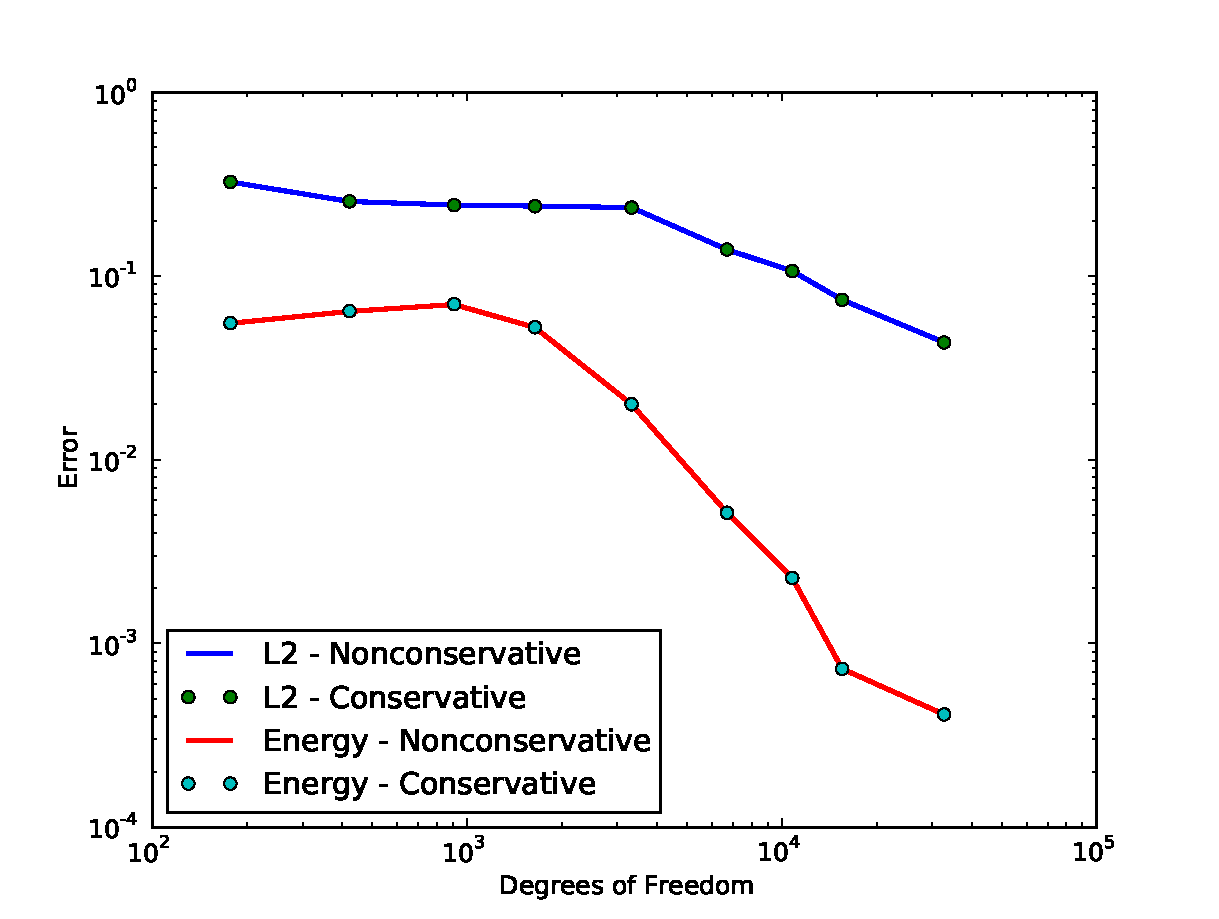
\includegraphics[width=\textwidth]{figs/Erickson/graphError.pdf}
\caption{With graph norm}
\label{fig:ericksonGraphError}
\end{subfigure}
\begin{subfigure}[t]{0.45\textwidth}
\centering
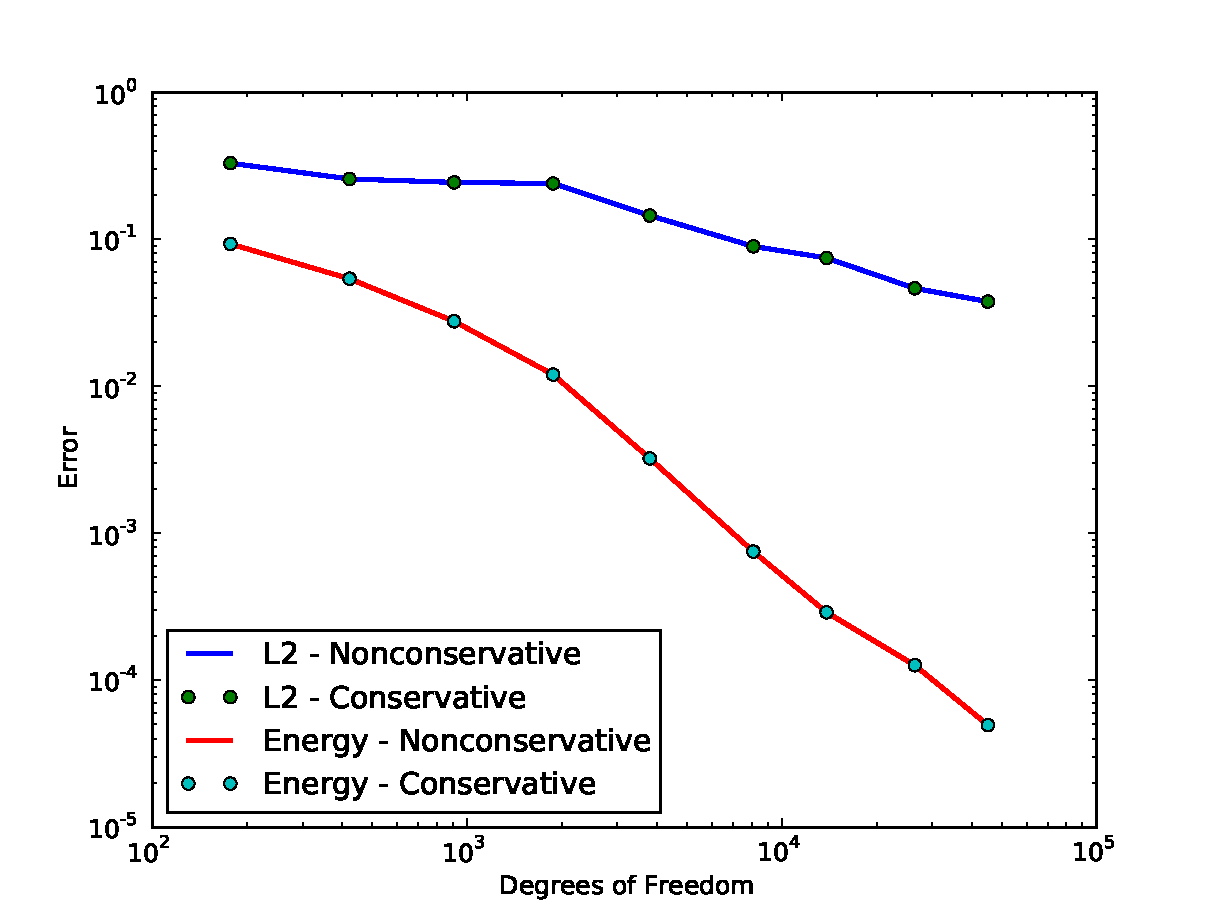
\includegraphics[width=\textwidth]{figs/Erickson/robustError.pdf}
\caption{With robust norm}
\label{fig:ericksonRobustError}
\end{subfigure}
\caption{Error in Erickson-Johnson solutions}
\end{figure}

We plot the flux imbalance errors in Figures \ref{fig:ericksonGraphFlux} and
\ref{fig:ericksonRobustFlux}. As expected, the element conservative
formulation brings these errors to the order of machine precision, but it is
worth pointing out that the flux imbalances for standard DPG are reasonable,
especially under refinement.

\begin{figure}
\centering
\begin{subfigure}[t]{0.45\textwidth}
\centering
\includegraphics[width=\textwidth]{figs/Erickson/graphFlux.pdf}
\caption{With graph norm}
\label{fig:ericksonGraphFlux}
\end{subfigure}
\begin{subfigure}[t]{0.45\textwidth}
\centering
\includegraphics[width=\textwidth]{figs/Erickson/robustFlux.pdf}
\caption{With robust norm}
\label{fig:ericksonRobustFlux}
\end{subfigure}
\caption{Flux imbalance in Erickson-Johnson solutions}
\end{figure}

\subsection{Skewed Convection-Diffusion Problem}
This is a standard convection-diffusion problem with a skewed convection
vector relative to the mesh. The problem setup is identical to the
Erickson-Johnson problems except that $\bbeta=(2,1)$. The following results
are for $\epsilon=10^{-4}$. 

On our initial mesh, we see no noticeable difference between conservative and
nonconservative results, though the choice of test norm affects things
dramatically. The graph norm produces a solution which is comparable to an L2
project of the exact solution. In this case, the field variable don't show the
very small boundary layer along the right and top surfaces, though a
visualization of the traces would show that the wall boundary condition is in
fact being enforced. As we refine, the field variables will begin to reflect
the boundary layer. On the other hand, the robust norm does show a boundary
layer being formed in the field variables. 

\begin{figure}
\centering
\begin{subfigure}[t]{0.45\textwidth}
\centering
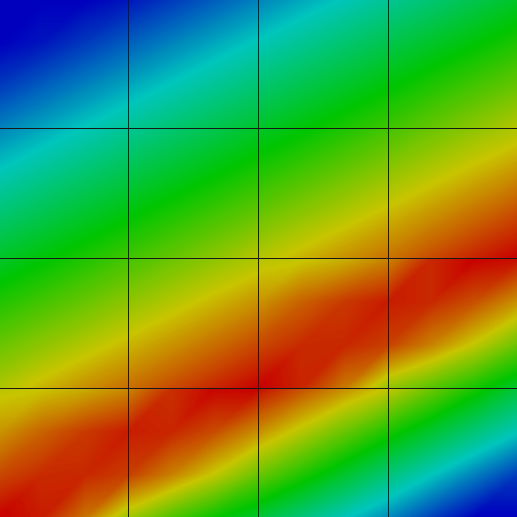
\includegraphics[width=\textwidth]{figs/Confusion/graph0c.png}
\caption{Conservative with graph norm}
\label{fig:confusionGraph0c}
\end{subfigure}
\begin{subfigure}[t]{0.45\textwidth}
\centering
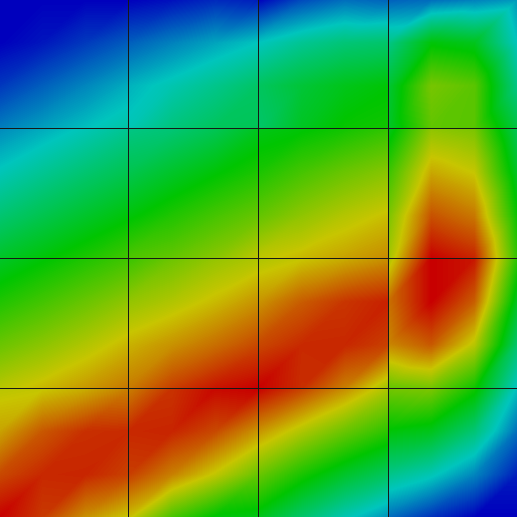
\includegraphics[width=\textwidth]{figs/Confusion/robust0c.png}
\caption{Conservative with robust norm}
\label{fig:confusionRobust0c}
\end{subfigure}
\caption{Skewed convection-diffusion problem with initial mesh}
\end{figure}

As we refine, the three results, nonconservative with graph or robust norm,
and conservative with graph norm converge to a an essentially identical
solution (to the eyeball norm), as represented by
Figure~\ref{fig:confusionGraph8c}. 

% However, the conservative formulation with
% the robust norm seems to exhibit some noise at the right wall as seen in
% Figure~\ref{fig:confusionRobust8c}.

\begin{figure}
\centering
\begin{subfigure}[t]{0.45\textwidth}
\centering
\includegraphics[width=\textwidth]{figs/Confusion/graph8c.png}
\includegraphics[width=\textwidth]{figs/Confusion/graph8c_mesh.png}
\caption{Conservative with graph norm}
\label{fig:confusionGraph8c}
\end{subfigure}
\begin{subfigure}[t]{0.45\textwidth}
\centering
\includegraphics[width=\textwidth]{figs/Confusion/robust8c.png}
\includegraphics[width=\textwidth]{figs/Confusion/robust8c_mesh.png}
\caption{Conservative with robust norm}
\label{fig:confusionRobust8c}
\end{subfigure}
\caption{Skewed convection-diffusion problem after 8 refinements}
\end{figure}

% If we zoom in on one of the noisy areas, as we do in
% Figure~\ref{fig:confusionRobust8c_zoom}, we see overshoots on the order of 32
% and undershoots on the order of -13, where the exact solution varies between 0
% and 1. The cause of these overshoots and undershoots is a little mystery,
% especially because they don't show up until 8 refinement steps in. We will
% explore this problem a little more when we look at the wedge problem.
% 
% \begin{figure}[h!]
% \centering
% 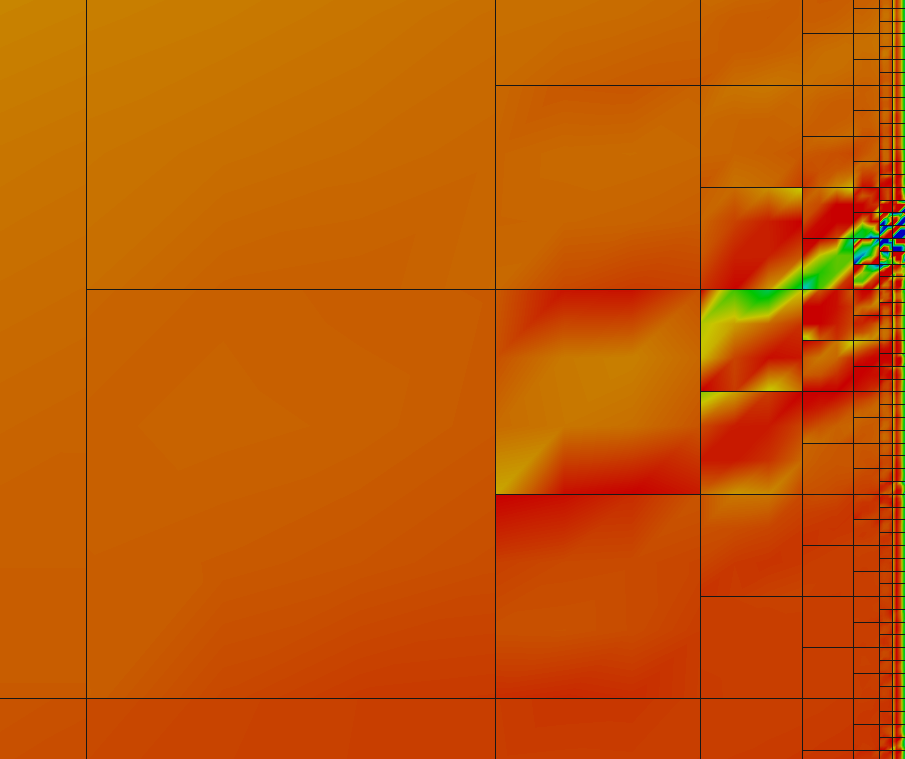
\includegraphics[width=0.6\textwidth]{figs/Confusion/robust8c_zoom.png}
% \caption{Zoomed in conservative skewed convection-diffusion problem after 8
% refinements}
% \label{fig:confusionRobust8c_zoom}
% \end{figure}

Finally, we plot the flux imbalances for the several methods in
Figure~\ref{fig:confusionGraphFlux} and Figure~\ref{fig:confusionRobustFlux}.
Interestingly, it appears the effectiveness of our local conservation
formulation drops as we refine with the graph norm.

\begin{figure}
\centering
\begin{subfigure}[t]{0.45\textwidth}
\centering
\includegraphics[width=\textwidth]{figs/Confusion/graphFlux.pdf}
\caption{With graph norm}
\label{fig:confusionGraphFlux}
\end{subfigure}
\begin{subfigure}[t]{0.45\textwidth}
\centering
\includegraphics[width=\textwidth]{figs/Confusion/robustFlux.pdf}
\caption{With robust norm}
\label{fig:confusionRobustFlux}
\end{subfigure}
\caption{Flux imbalance in skewed confusion solutions}
\end{figure}

\subsection{Double Glazing Problem}
This nominal problem definition takes the same unit square domain with 
\[
\bbeta=\binom{2(2y-1)(1-(2x-1)^2)}{-2(2x-1)(1-(2y-1)^2)}\,;\quad f=0\,;\quad
\hat u=
\begin{cases}
1 & \mbox{on }\Gamma_{right}\\
0 & \mbox{else }
\end{cases}\,,
\]
except that this definition for the boundary is not legal for $\hat u\in
H^{\frac{1}{2}}(\Gamma_h)$ which is continuous. Therefore we use a ramp of
width $\sqrt{\epsilon}$ on the right edge to go from 0 to 1. The following
results are for $\epsilon=10^{-2}$. Note that $\bbeta=(0,0)^T$ at the center
of the domain.

The choice of test norm appears to have a small effect on the choice mesh
refinement choices as shown in Figure~\ref{fig:doubleglazing}. Other than
that, the conservative and nonconservative solutions behave almost exactly to
the eye. The flux imbalances in Figure~\ref{fig:doubleglazing_flux} are what
we would expect. The nonconservative formulation appears to become more
conservative with refinement.

\begin{figure}
\centering
\begin{subfigure}[t]{0.45\textwidth}
\centering
\includegraphics[width=\textwidth]{figs/DoubleGlazing/graph6c.png}
\caption{Conservative with graph norm}
\label{fig:doubleglazingGraph6c}
\end{subfigure}
\begin{subfigure}[t]{0.45\textwidth}
\centering
\includegraphics[width=\textwidth]{figs/DoubleGlazing/robust6c.png}
\caption{Conservative with robust norm}
\label{fig:doubleglazingRobust6c}
\end{subfigure}
\caption{Double glazing problem after 6 refinements}
\label{fig:doubleglazing}
\end{figure}

\begin{figure}
\centering
\begin{subfigure}[t]{0.45\textwidth}
\centering
\includegraphics[width=\textwidth]{figs/DoubleGlazing/graphFlux.pdf}
\caption{With graph norm}
\label{fig:doubleglazingGraphFlux}
\end{subfigure}
\begin{subfigure}[t]{0.45\textwidth}
\centering
\includegraphics[width=\textwidth]{figs/DoubleGlazing/robustFlux.pdf}
\caption{With robust norm}
\label{fig:doubleglazingRobustFlux}
\end{subfigure}
\caption{Flux imbalance in double glazing solutions}
\label{fig:doubleglazing_flux}
\end{figure}

\subsection{Vortex Problem}
This problem models a mildly diffusive vortex convecting fluid in a circle. We
deal with domain $\Omega=[-1,1]^2$ with $\epsilon=10^{-4}$, $\bbeta=(-y,x)^T$,
and $f=0$. Note that $\bbeta=0$ at the domain center. We have an inflow
boundary condition when $\bbeta\cdot\mathbf{n}<0$, in which case we set $\hat
t=\bbeta\cdot\mathbf{n}\cdot u_0$ where
$u_0=\frac{\sqrt{x^2+y^2}-1}{\sqrt{2}-1}$ which will vary from 0 at the center
of boundary edges to 1 at corners. We don't enforce an outflow boundary.

Each of the four methods seems to have it's own specific refinement pattern,
but in general we can see that the nonconservative formulations seem to place
much more refinements in the center of the vortex where the solution is
constant. The conservative formulations seem to recognize that more error is
concentrated on the edges of the vortex where we have a sharp change from
constant values to linear growth in terms of radius. Again we see that
standard DPG appears to approach conservation with refinement, and
unfortunately the conservative formulation appears to be losing enforcement
under the robust norm.

\begin{figure}
\centering
\begin{subfigure}[t]{0.45\textwidth}
\centering
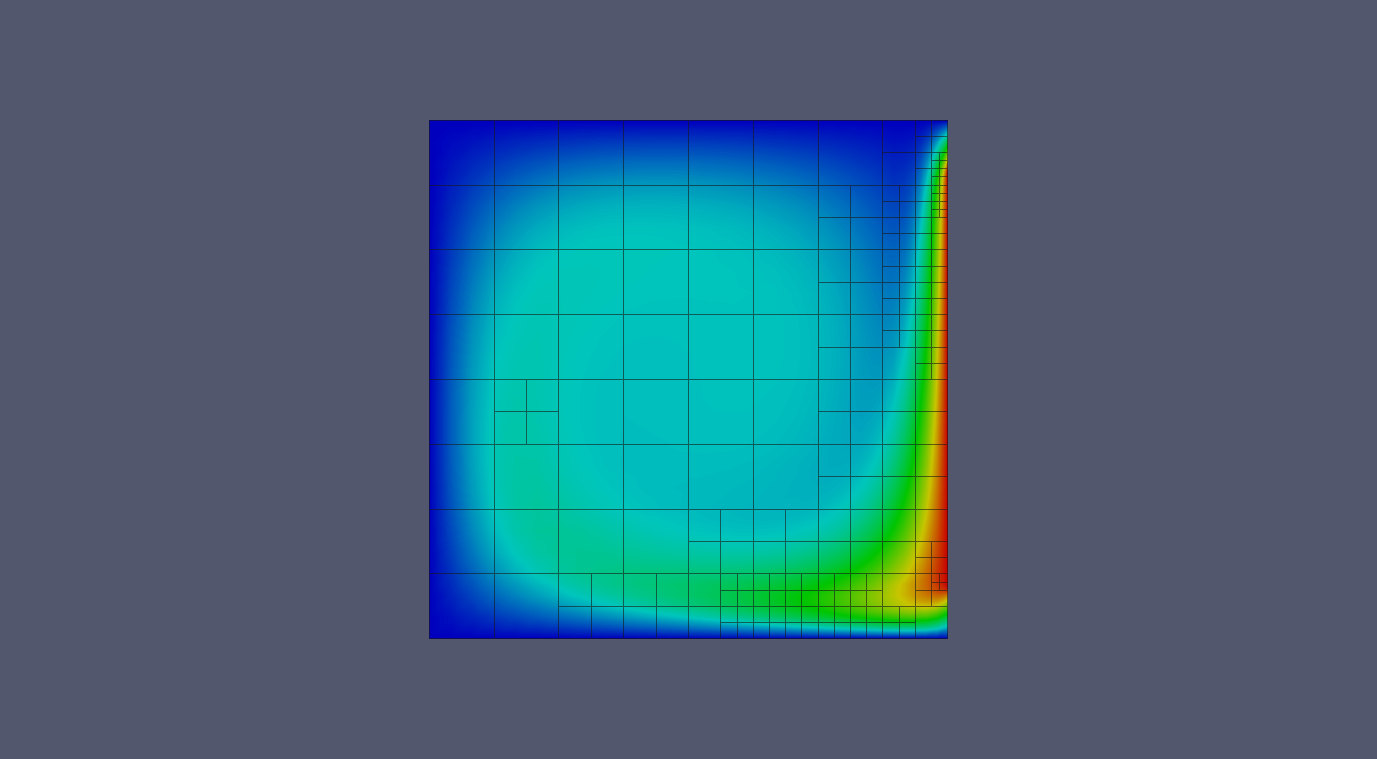
\includegraphics[width=\textwidth]{figs/Vortex/graph6nc.png}
\caption{Nonconservative with graph norm}
\label{fig:vortexGraph6nc}
\end{subfigure}
\begin{subfigure}[t]{0.45\textwidth}
\centering
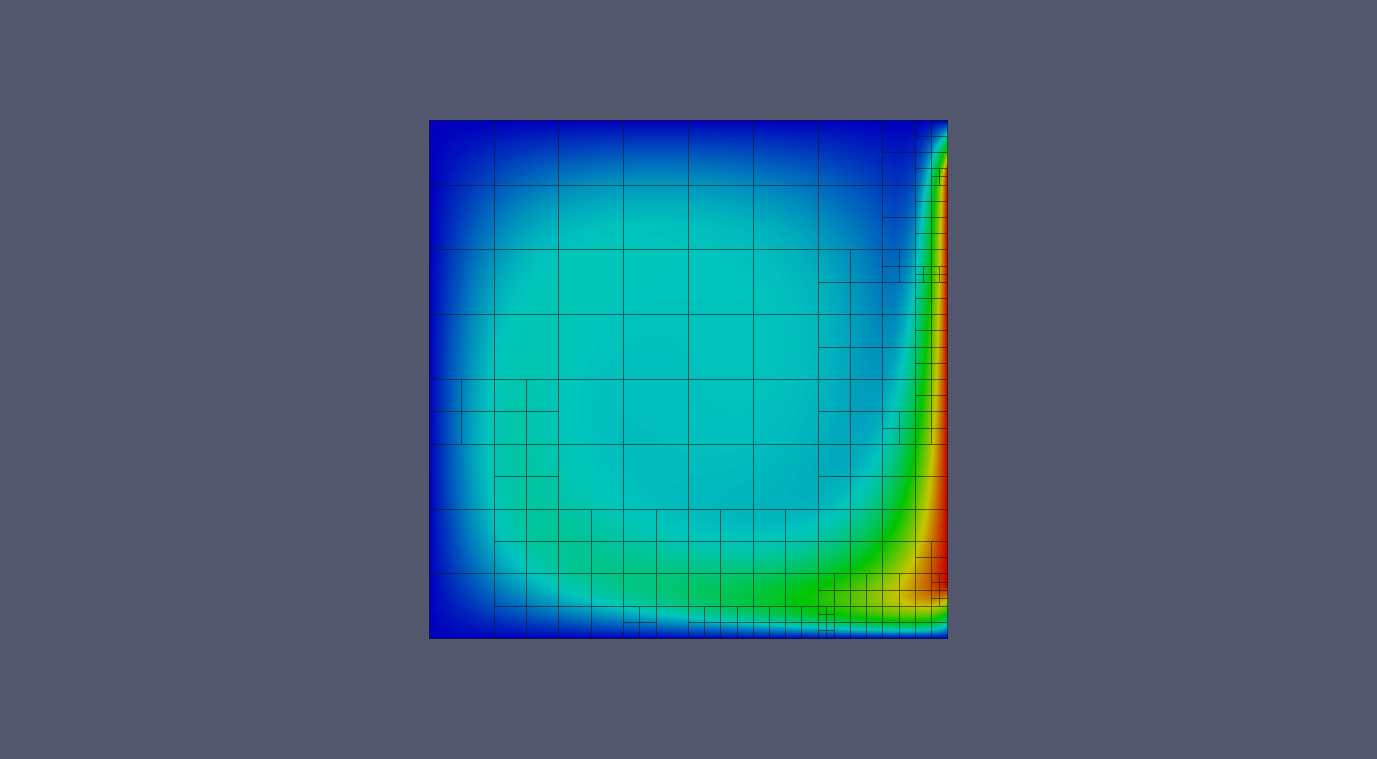
\includegraphics[width=\textwidth]{figs/Vortex/robust6nc.png}
\caption{Nonconservative with robust norm}
\label{fig:vortexRobust6nc}
\end{subfigure}
\begin{subfigure}[t]{0.45\textwidth}
\centering
\includegraphics[width=\textwidth]{figs/Vortex/graph6c.png}
\caption{Conservative with graph norm}
\label{fig:vortexGraph6c}
\end{subfigure}
\begin{subfigure}[t]{0.45\textwidth}
\centering
\includegraphics[width=\textwidth]{figs/Vortex/robust6c.png}
\caption{Conservative with robust norm}
\label{fig:vortexRobust6c}
\end{subfigure}
\caption{Vortex problem after 6 refinements}
\label{fig:vortex}
\end{figure}

\begin{figure}
\centering
\begin{subfigure}[t]{0.45\textwidth}
\centering
\includegraphics[width=\textwidth]{figs/Vortex/graphFlux.pdf}
\caption{With graph norm}
\label{fig:vortexGraphFlux}
\end{subfigure}
\begin{subfigure}[t]{0.45\textwidth}
\centering
\includegraphics[width=\textwidth]{figs/Vortex/robustFlux.pdf}
\caption{With robust norm}
\label{fig:vortexRobustFlux}
\end{subfigure}
\caption{Flux imbalance in vortex solutions}
\label{fig:vortex_flux}
\end{figure}

\subsection{Wedge Problem}
We devised this problem to examine some of the issues we were having blow up
of the solution under the robust test norm. The domain is a rectangle
$[-0.5,0.5]\times[-1,0.5]$ where the triangle connecting the bottom edges with
the origin at $(0,0)$ is removed. The convection vector $\bbeta=(1,0)^T$,
$\epsilon=10^{-1}$, and we apply boundary conditions $\hat t=0$ on the left
inflow edge, $\hat u=0$ on the top edge, $\bbeta\cdot\mathbf{n}\cdot\hat
u-\hat t=\sigma_n=0$ on the right outflow edge, $\hat u=1$ on the leading edge
of the wedge, and $\hat t=\bbeta\cdot\mathbf{n}\cdot 1$ on the trailing edge
of the wedge.

When the colorscale is scaled from 0 to 1, the macro view of all of the
solutions looks nearly identical as seen in Figure~\ref{fig:wedge}. However,
we start to see some differences in the refinement patterns in
Figure~\ref{fig:wedge_mesh} indicating that the various methods distribute
error in different ways. We see more evidence of this when we zoom in on the
tip of the wedge where we get a change in boundary conditions. The graph norm
solutions don't exhibit any significant problems here. The nonconservative and
conservative solutions vary smoothly in the range $(-0.00127, 1.03)$, plus or
minus some less significant digits. The nonconservative robust solution jumps
from -19.6 to 20.3 at the tip, though this appears to be a very localized
phenominon. Adding local conservation appears to exacerbate this situation as
the solution varies from -20.0 to 23.2 and appears to polute a larger area of
the problem. We implemented a crude hp-adaptive refinement strategy in order
to try to resolve any singularities present in the solution. If the cell
measure dips below $5\times10^{-4}$, we switch from h-adaptivity to
p-adaptivity. Figure~\ref{fig:wedge_poly} shows the resultant polynomial
orders after refinement. It really appears that the apparent singularities in
the robust solutions are not physical phenomena that just need resolution, but
a weakness in the method with the robust test norm.

We plot the flux imbalances in Figure~\ref{fig:wedge_flux}. Despite the
extreme overshoots and undershoots in the conservative method with the robust
test norm, we still appear to maintain acceptable levels of conservation.

\begin{figure}
\centering
\begin{subfigure}[t]{0.4\textwidth}
\centering
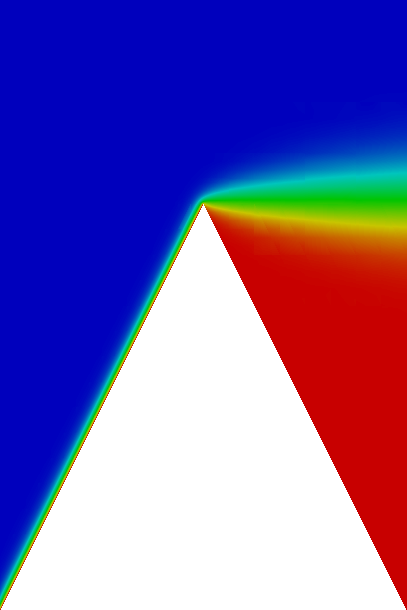
\includegraphics[width=\textwidth]{figs/Wedge/graph16nc.png}
\caption{Nonconservative with graph norm}
\label{fig:wedgeGraph16nc}
\end{subfigure}
\begin{subfigure}[t]{0.4\textwidth}
\centering
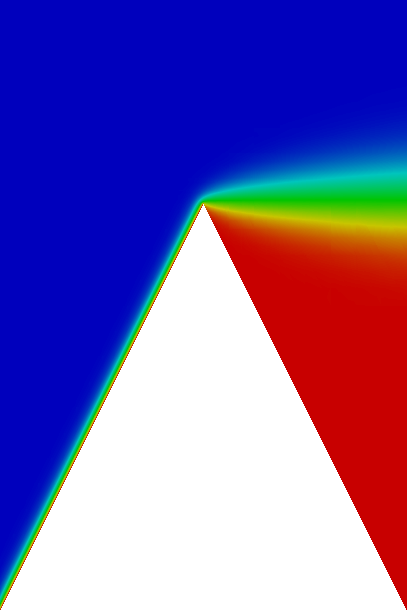
\includegraphics[width=\textwidth]{figs/Wedge/robust16nc.png}
\caption{Nonconservative with robust norm}
\label{fig:wedgeRobust16nc}
\end{subfigure}
\begin{subfigure}[t]{0.4\textwidth}
\centering
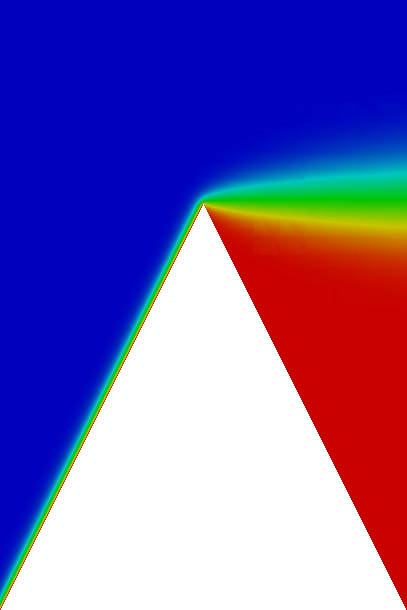
\includegraphics[width=\textwidth]{figs/Wedge/graph16c.png}
\caption{Conservative with graph norm}
\label{fig:wedgeGraph16c}
\end{subfigure}
\begin{subfigure}[t]{0.4\textwidth}
\centering
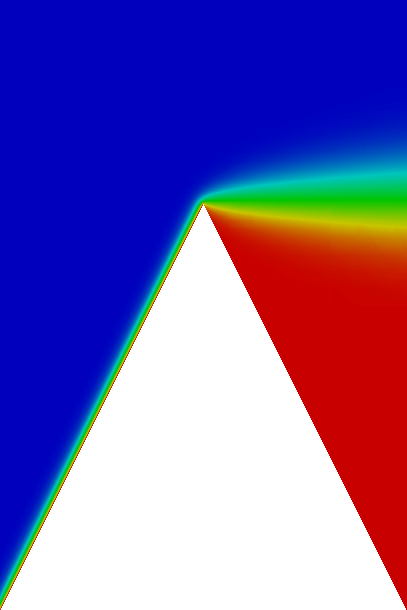
\includegraphics[width=\textwidth]{figs/Wedge/robust16c.png}
\caption{Conservative with robust norm}
\label{fig:wedgeRobust16c}
\end{subfigure}
\caption{Wedge problem after 16 refinements}
\label{fig:wedge}
\end{figure}

\begin{figure}
\centering
\begin{subfigure}[t]{0.4\textwidth}
\centering
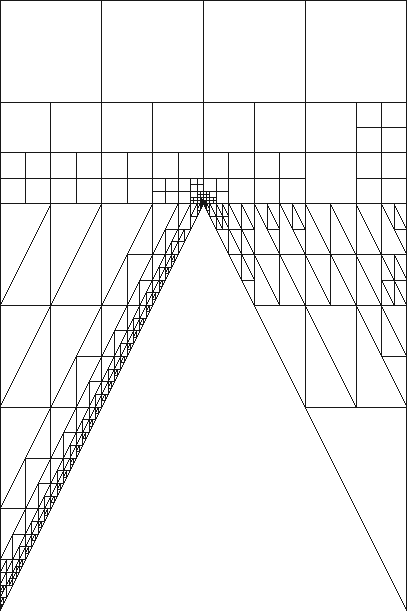
\includegraphics[width=\textwidth]{figs/Wedge/graph16nc_mesh.png}
\caption{Nonconservative with graph norm}
\label{fig:wedgeGraph16nc_mesh}
\end{subfigure}
\begin{subfigure}[t]{0.4\textwidth}
\centering
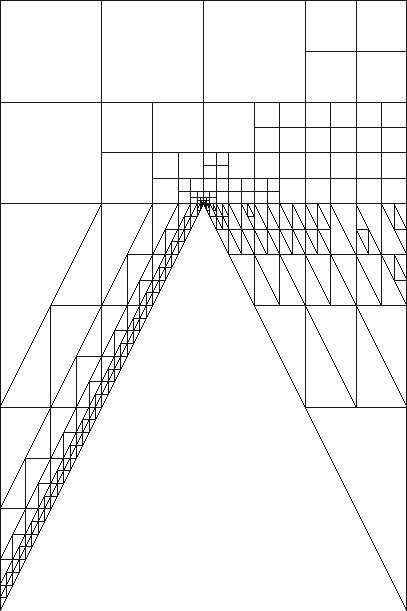
\includegraphics[width=\textwidth]{figs/Wedge/robust16nc_mesh.png}
\caption{Nonconservative with robust norm}
\label{fig:wedgeRobust16nc_mesh}
\end{subfigure}
\begin{subfigure}[t]{0.4\textwidth}
\centering
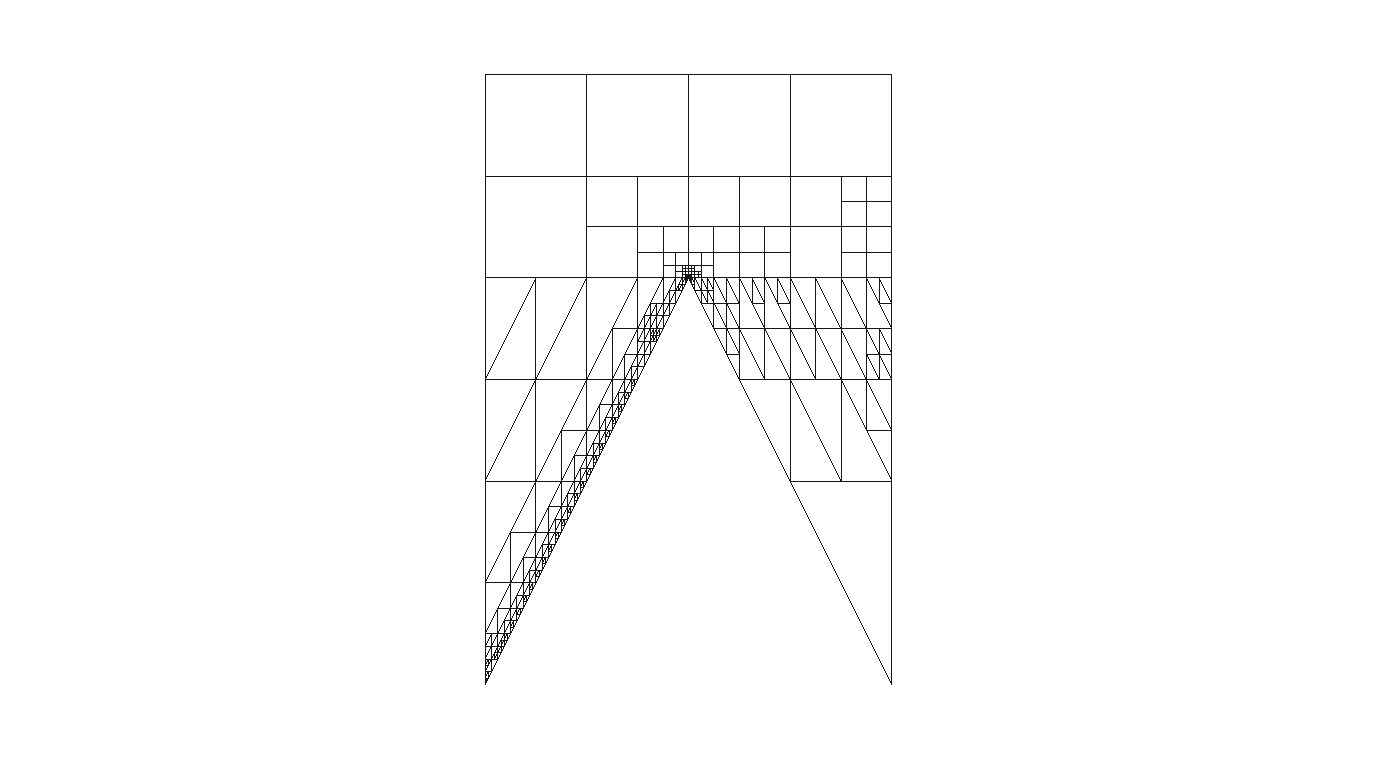
\includegraphics[width=\textwidth]{figs/Wedge/graph16c_mesh.png}
\caption{Conservative with graph norm}
\label{fig:wedgeGraph16c_mesh}
\end{subfigure}
\begin{subfigure}[t]{0.4\textwidth}
\centering
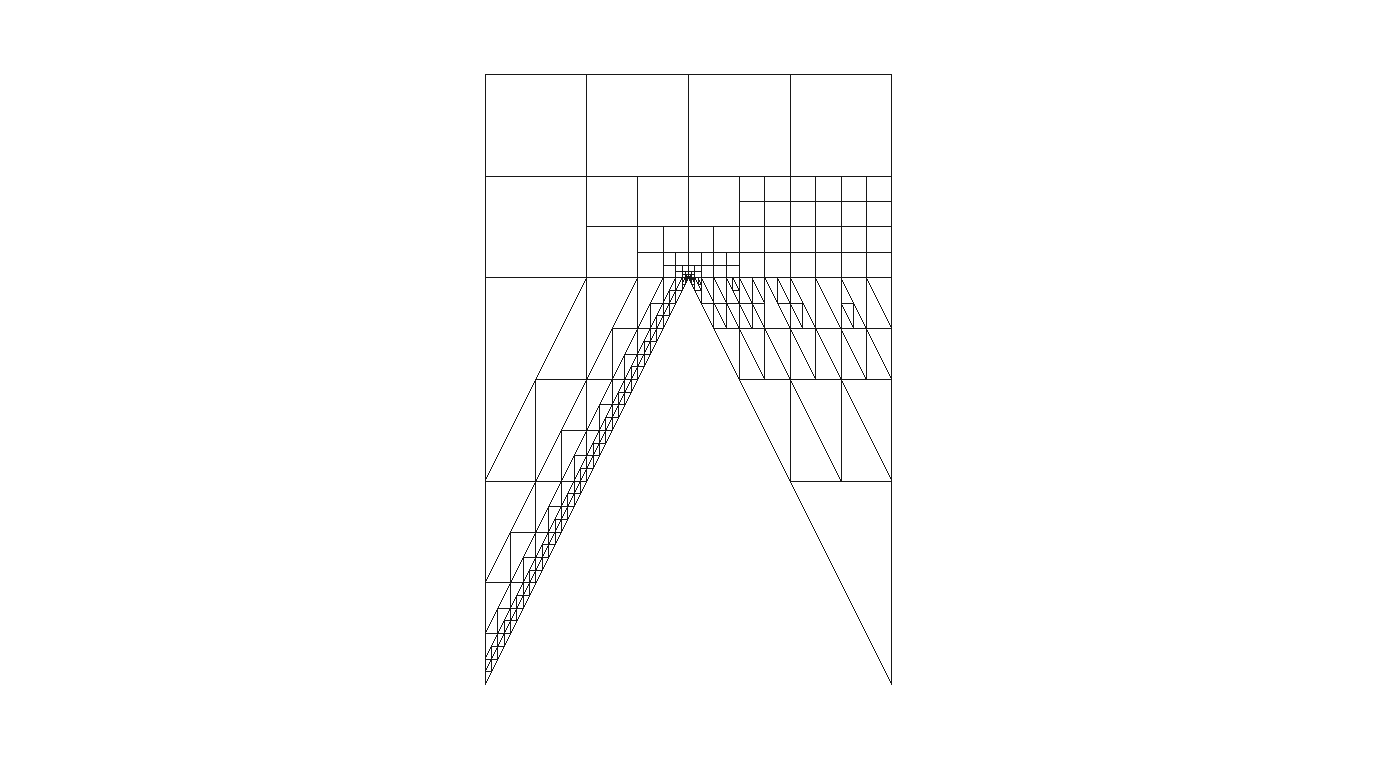
\includegraphics[width=\textwidth]{figs/Wedge/robust16c_mesh.png}
\caption{Conservative with robust norm}
\label{fig:wedgeRobust16c_mesh}
\end{subfigure}
\caption{Wedge problem mesh after 16 refinements}
\label{fig:wedge_mesh}
\end{figure}

\begin{figure}
\centering
\begin{subfigure}[t]{0.45\textwidth}
\centering
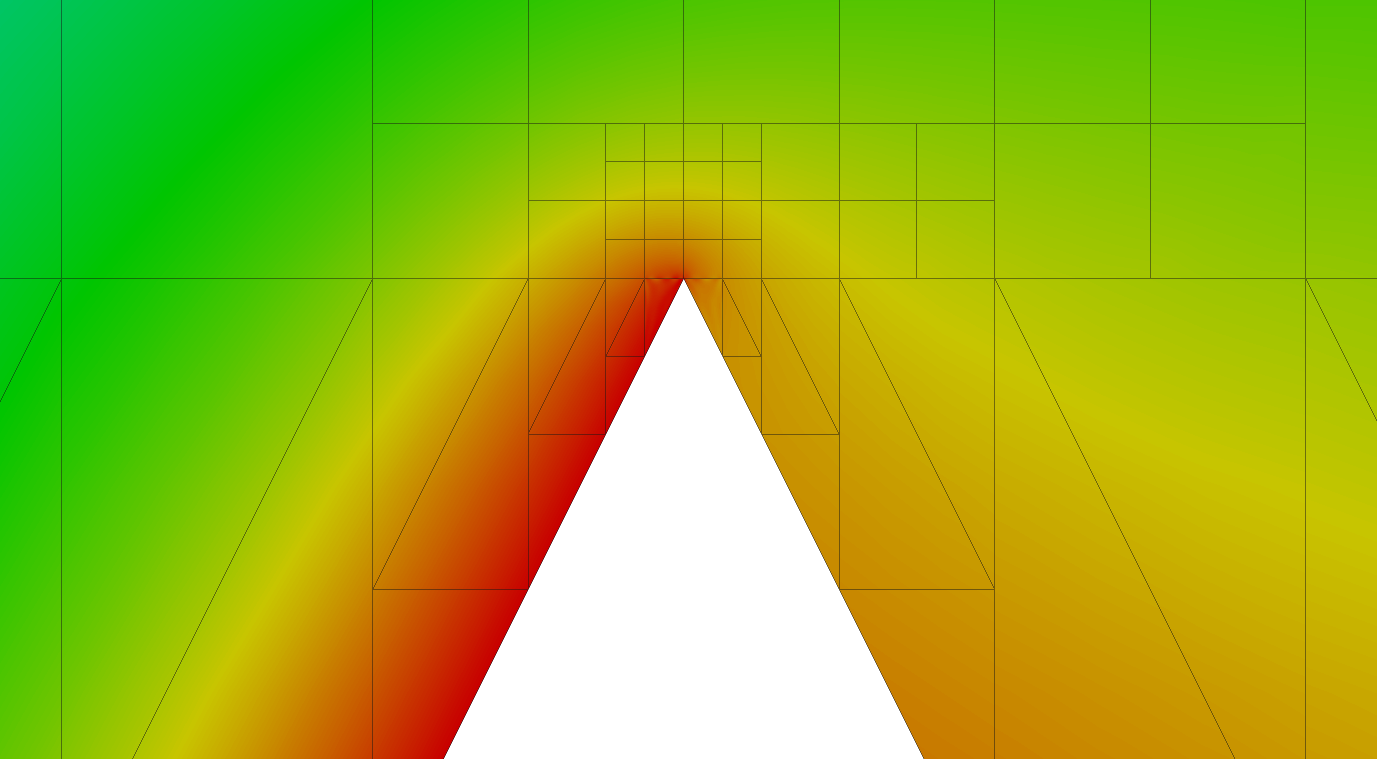
\includegraphics[width=\textwidth]{figs/Wedge/graph16nc_zoom.png}
\caption{Nonconservative with graph norm}
\label{fig:wedgeGraph16nc_zoom}
\end{subfigure}
\begin{subfigure}[t]{0.45\textwidth}
\centering
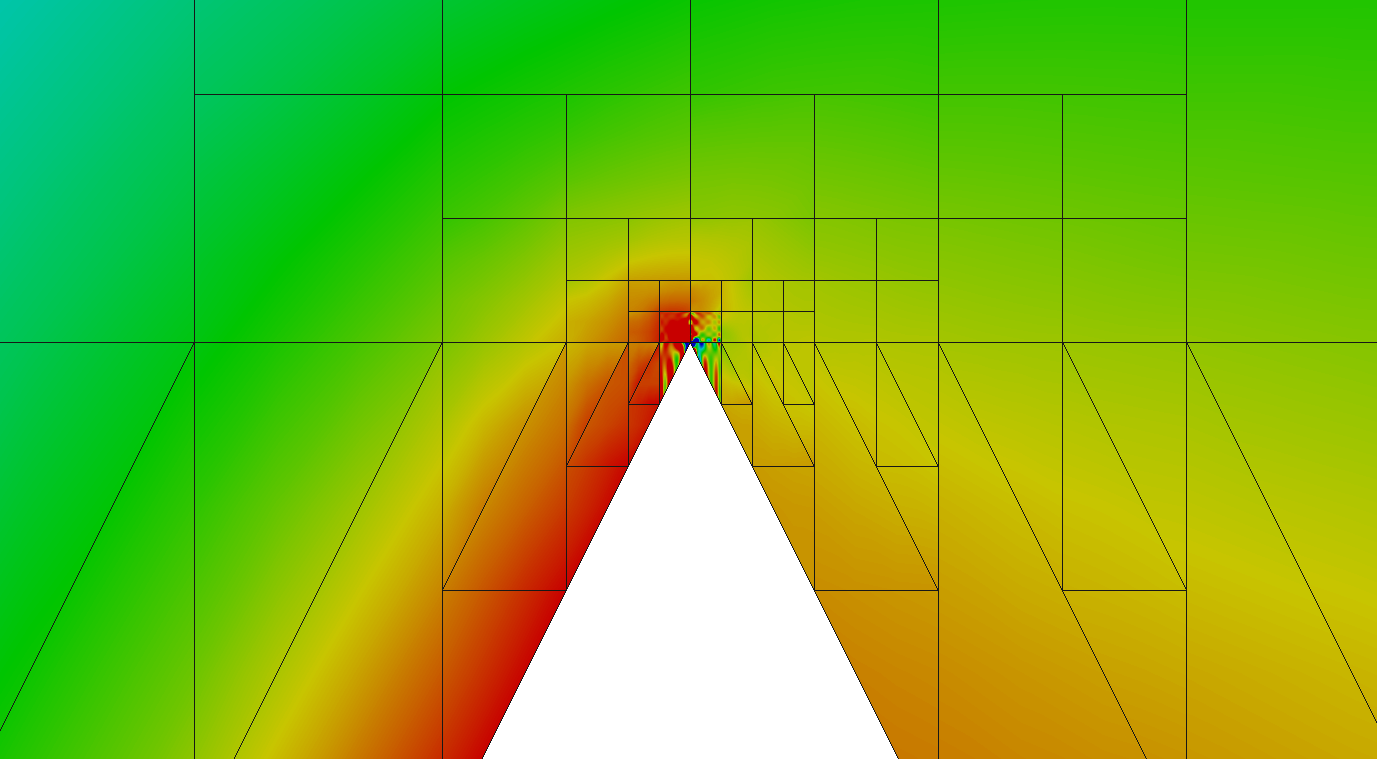
\includegraphics[width=\textwidth]{figs/Wedge/robust16nc_zoom.png}
\caption{Nonconservative with robust norm}
\label{fig:wedgeRobust16nc_zoom}
\end{subfigure}
\begin{subfigure}[t]{0.45\textwidth}
\centering
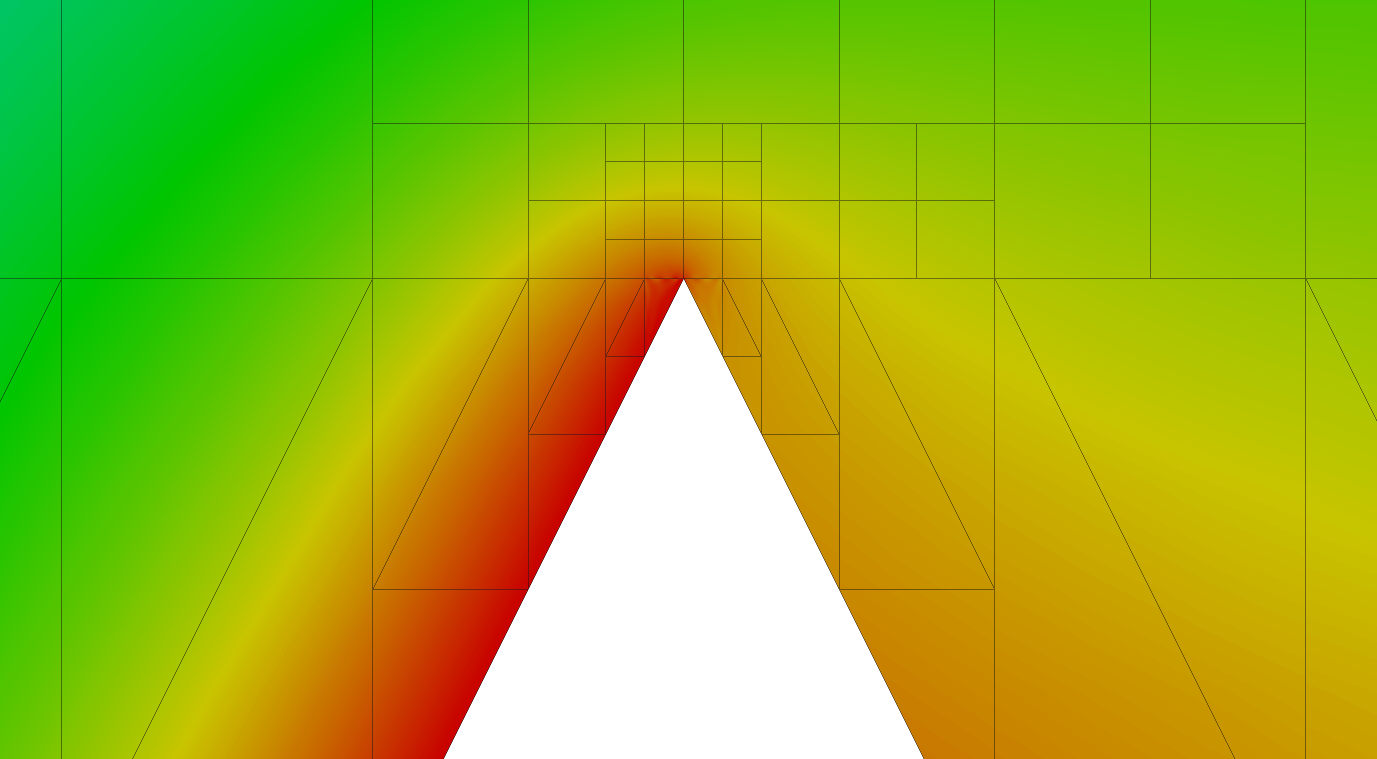
\includegraphics[width=\textwidth]{figs/Wedge/graph16c_zoom.png}
\caption{Conservative with graph norm}
\label{fig:wedgeGraph16c_zoom}
\end{subfigure}
\begin{subfigure}[t]{0.45\textwidth}
\centering
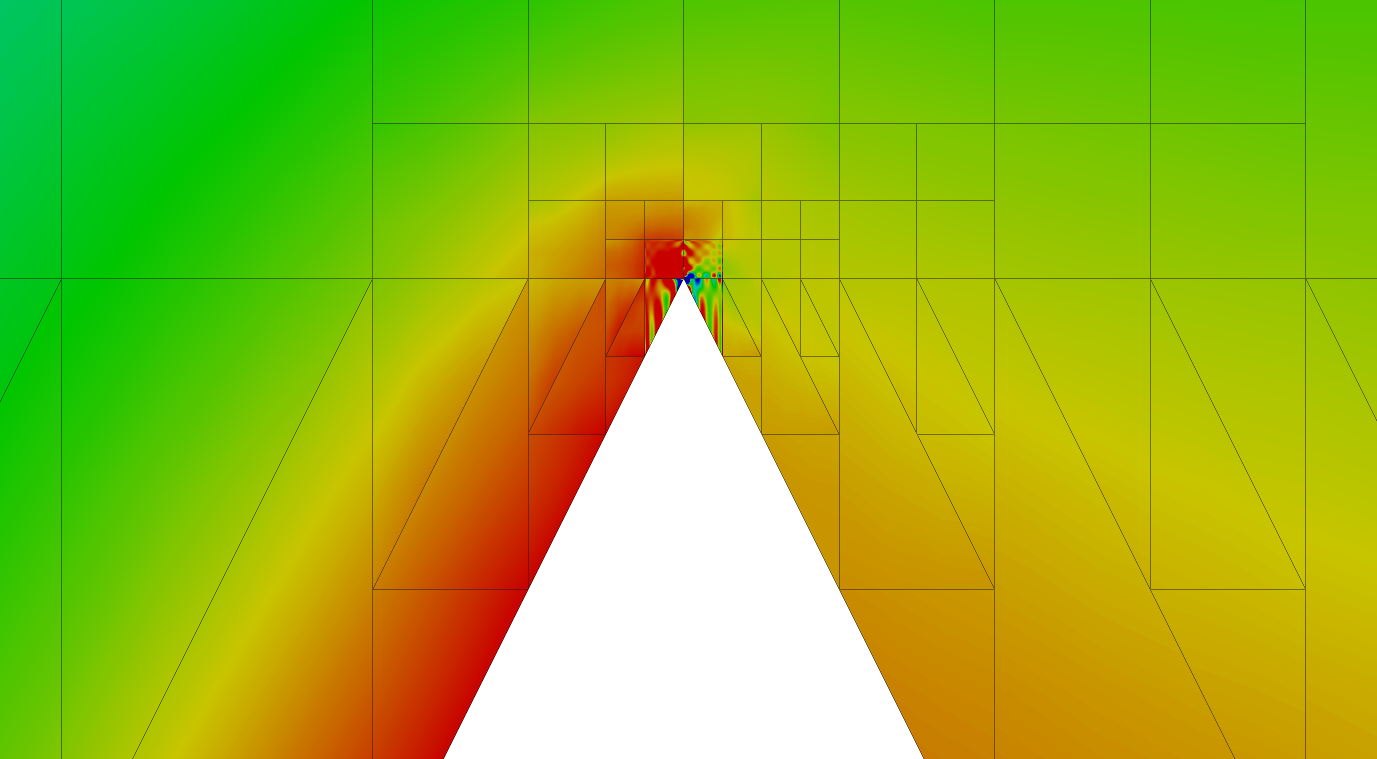
\includegraphics[width=\textwidth]{figs/Wedge/robust16c_zoom.png}
\caption{Conservative with robust norm}
\label{fig:wedgeRobust16c_zoom}
\end{subfigure}
\caption{Wedge problem zoomed in after 16 refinements}
\label{fig:wedge_zoom}
\end{figure}

\begin{figure}
\centering
\begin{subfigure}[t]{0.45\textwidth}
\centering
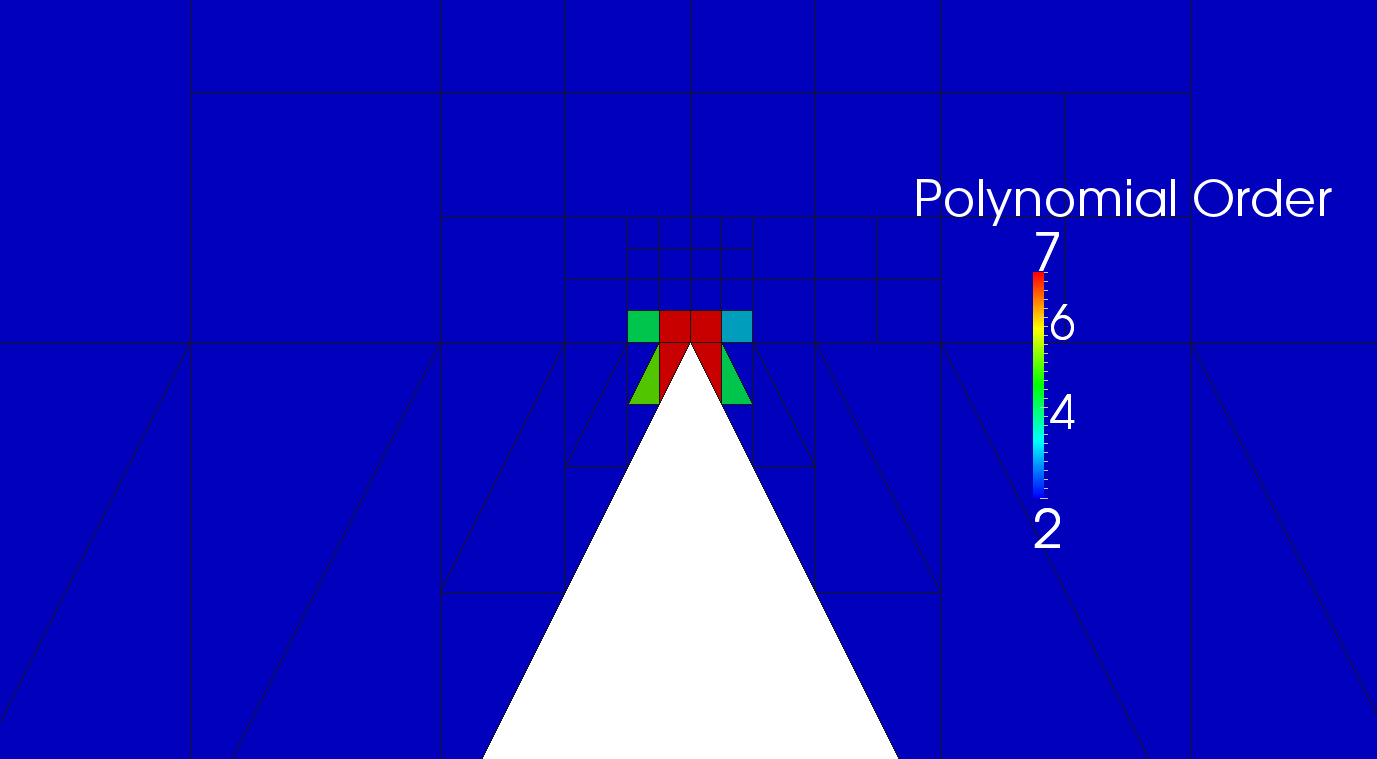
\includegraphics[width=\textwidth]{figs/Wedge/graph16nc_poly.png}
\caption{Nonconservative with graph norm}
\label{fig:wedgeGraph16nc_poly}
\end{subfigure}
\begin{subfigure}[t]{0.45\textwidth}
\centering
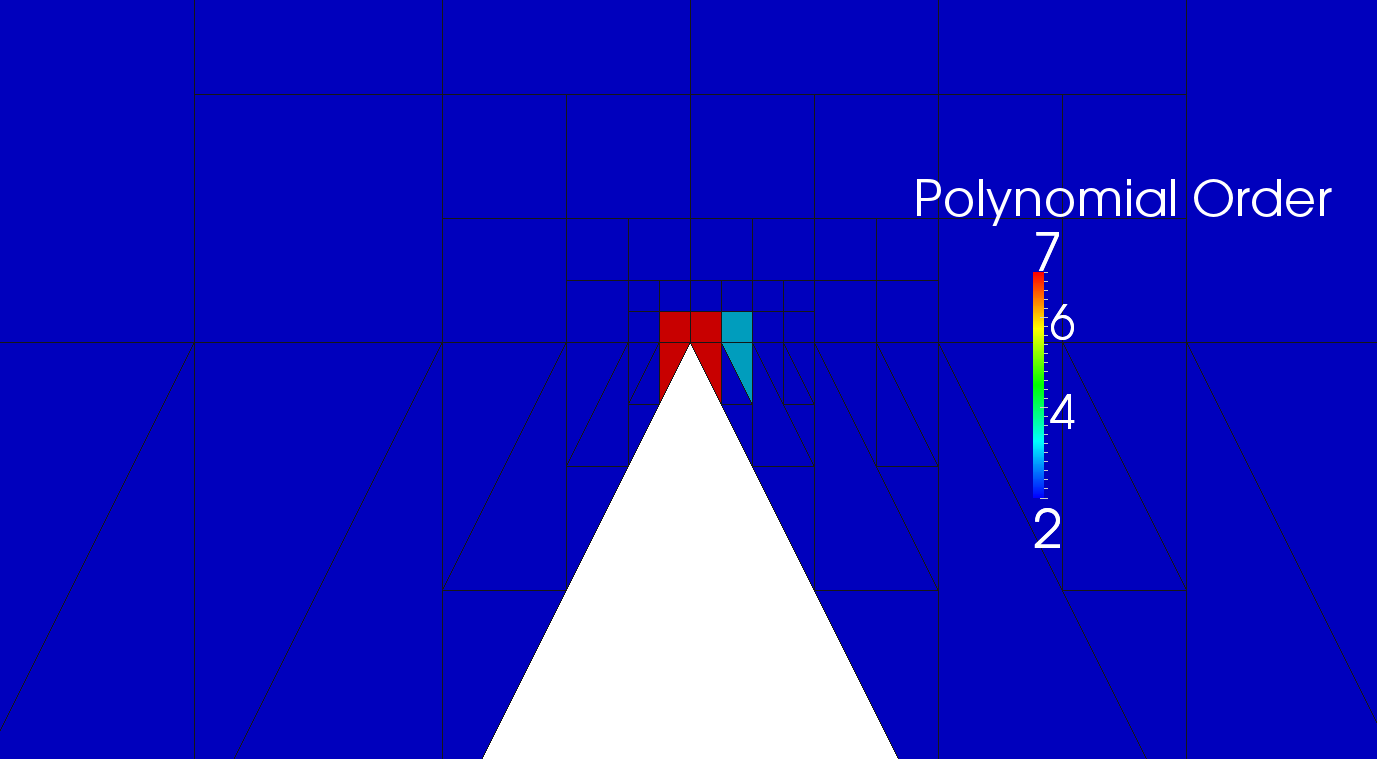
\includegraphics[width=\textwidth]{figs/Wedge/robust16nc_poly.png}
\caption{Nonconservative with robust norm}
\label{fig:wedgeRobust16nc_poly}
\end{subfigure}
\begin{subfigure}[t]{0.45\textwidth}
\centering
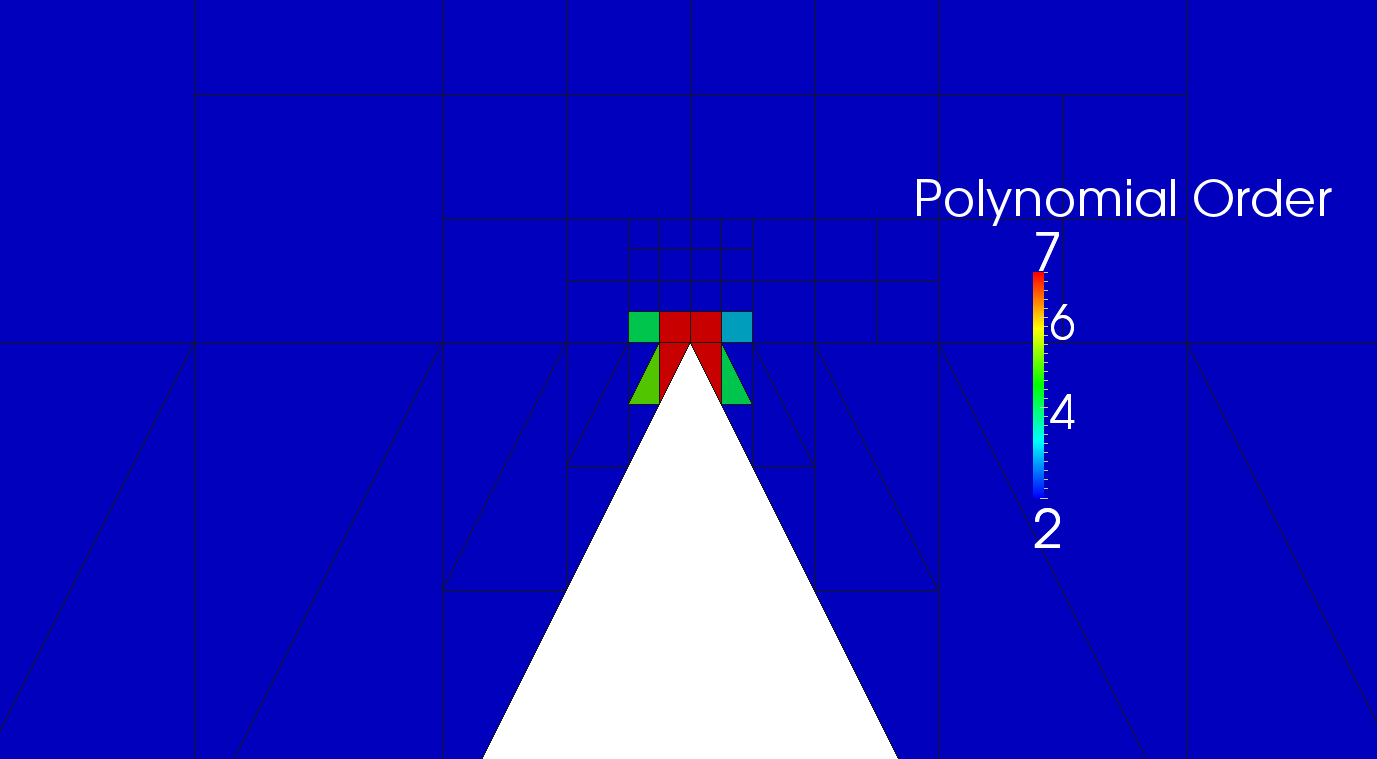
\includegraphics[width=\textwidth]{figs/Wedge/graph16c_poly.png}
\caption{Conservative with graph norm}
\label{fig:wedgeGraph16c_poly}
\end{subfigure}
\begin{subfigure}[t]{0.45\textwidth}
\centering
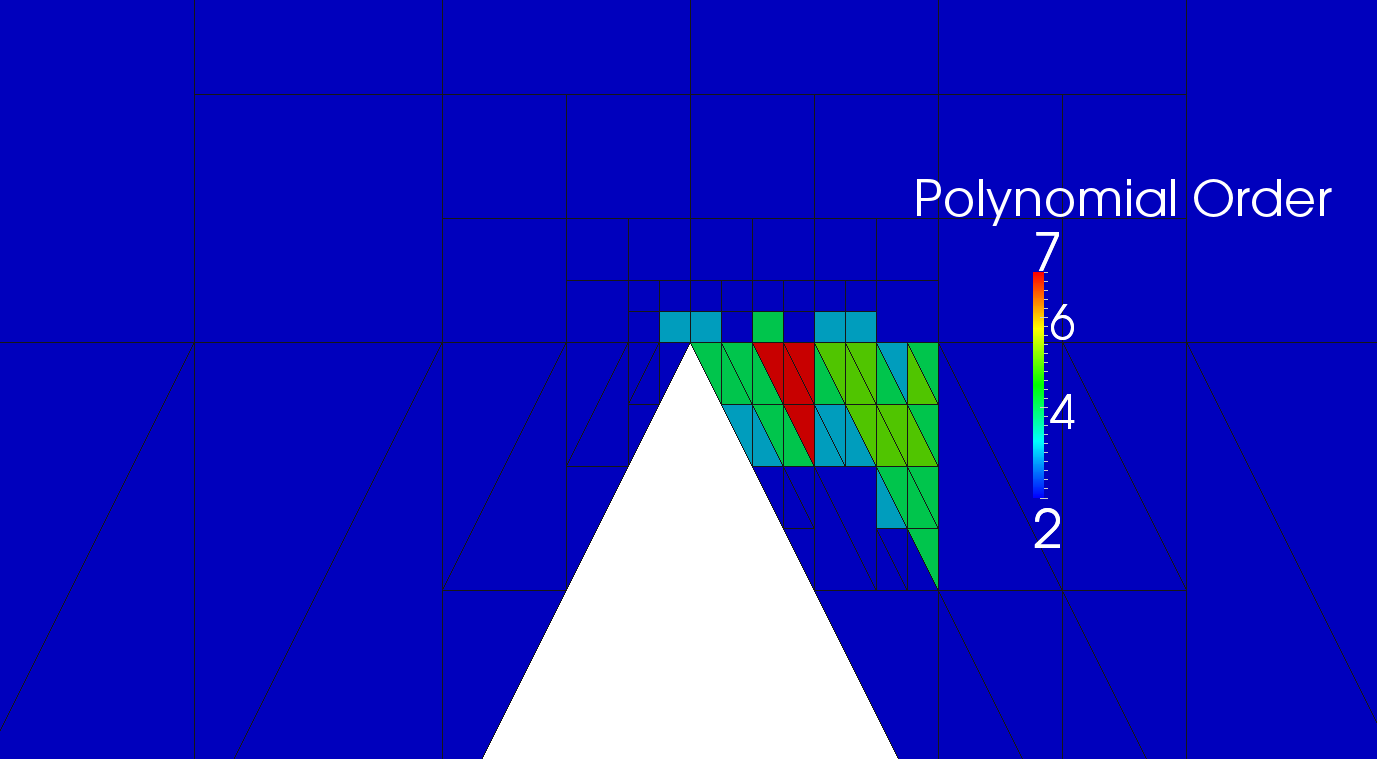
\includegraphics[width=\textwidth]{figs/Wedge/robust16c_poly.png}
\caption{Conservative with robust norm}
\label{fig:wedgeRobust16c_poly}
\end{subfigure}
\caption{Wedge problem poly after 16 refinements}
\label{fig:wedge_poly}
\end{figure}

\begin{figure}
\centering
\begin{subfigure}[t]{0.45\textwidth}
\centering
\includegraphics[width=\textwidth]{figs/Wedge/graphFlux.pdf}
\caption{With graph norm}
\label{fig:wedgeGraphFlux}
\end{subfigure}
\begin{subfigure}[t]{0.45\textwidth}
\centering
\includegraphics[width=\textwidth]{figs/Wedge/robustFlux.pdf}
\caption{With robust norm}
\label{fig:wedgeRobustFlux}
\end{subfigure}
\caption{Flux imbalance in wedge solutions}
\label{fig:wedge_flux}
\end{figure}

\subsection{Inner Layer Problem}

\begin{figure}
\centering
\begin{subfigure}[t]{0.45\textwidth}
\centering
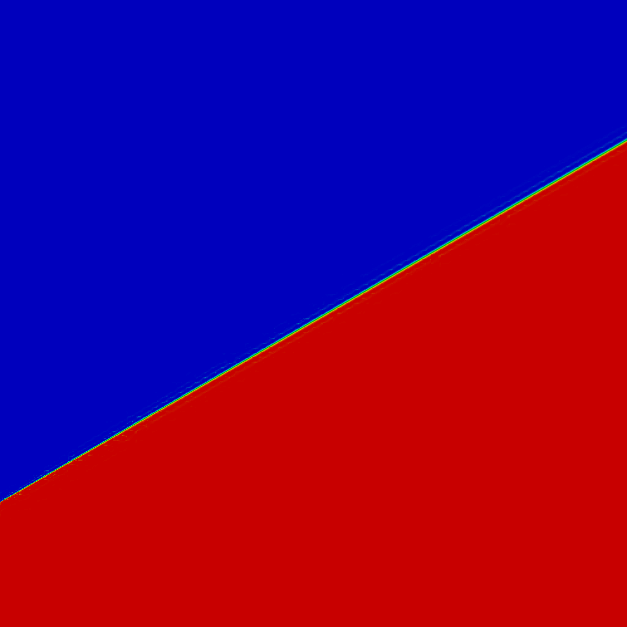
\includegraphics[width=\textwidth]{figs/InnerLayer/graph8nc.png}
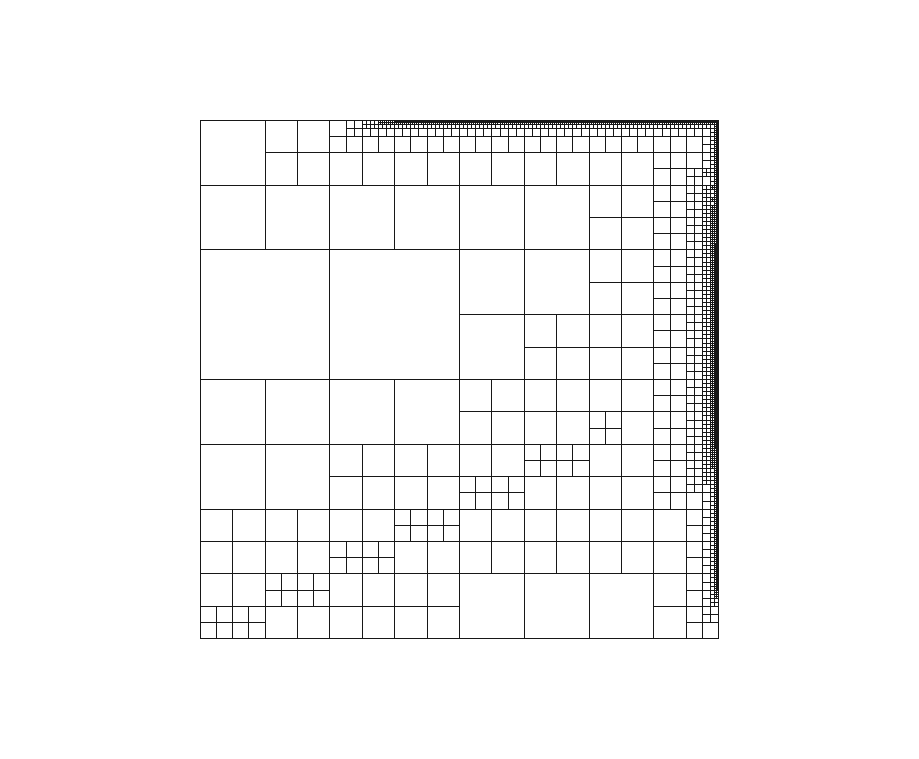
\includegraphics[width=\textwidth]{figs/InnerLayer/graph8nc_mesh.png}
\caption{Nonconservative with graph norm}
\label{fig:innerlayerGraph18nc}
\end{subfigure}
\begin{subfigure}[t]{0.45\textwidth}
\centering
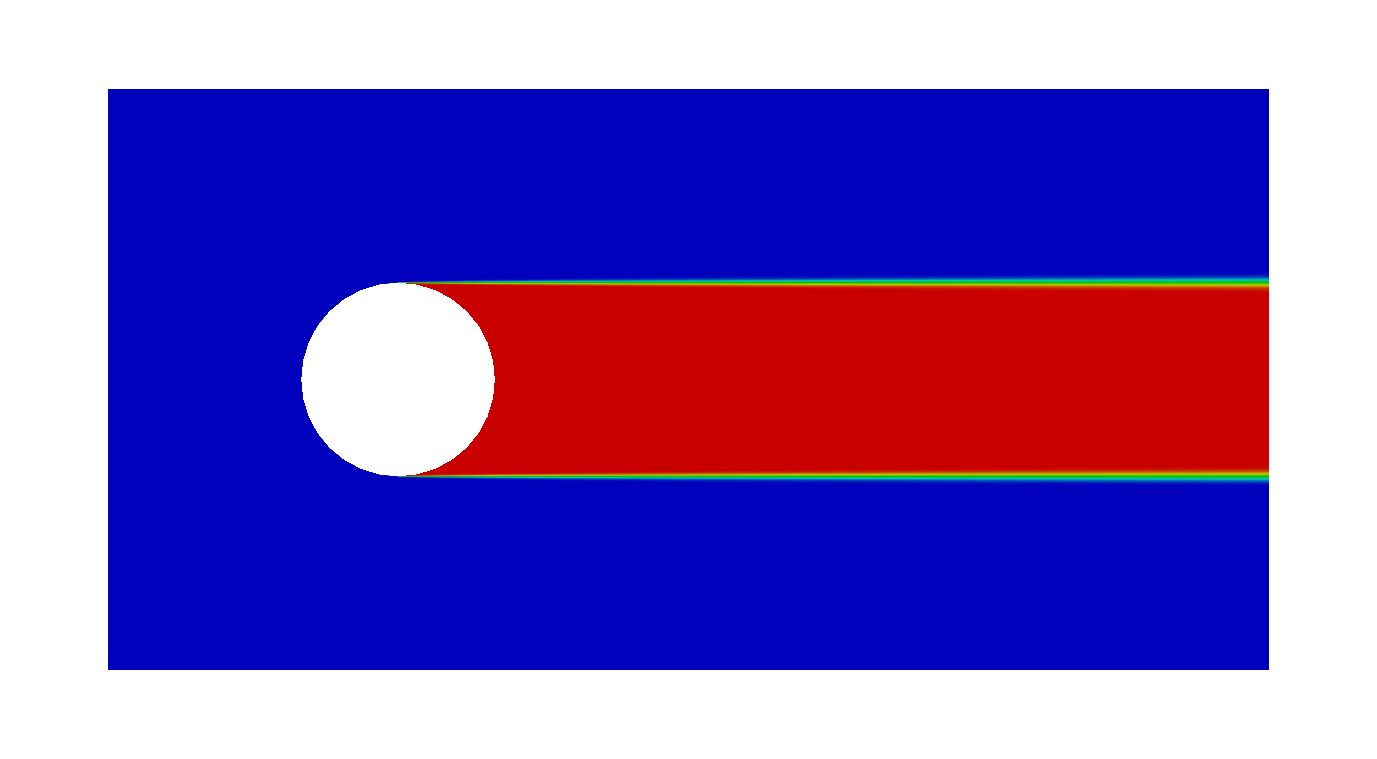
\includegraphics[width=\textwidth]{figs/InnerLayer/robust8nc.png}
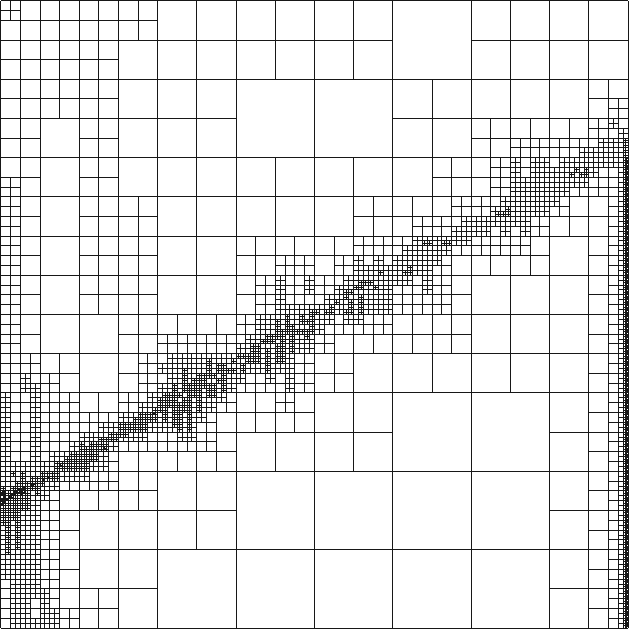
\includegraphics[width=\textwidth]{figs/InnerLayer/robust8nc_mesh.png}
\caption{Nonconservative with robust norm}
\label{fig:innerlayerRobust18nc}
\end{subfigure}
\caption{Inner layer problem after 8 refinements}
\label{fig:innerlayer8nc}
\end{figure}

\begin{figure}
\centering
\begin{subfigure}[t]{0.45\textwidth}
\centering
\includegraphics[width=\textwidth]{figs/InnerLayer/graph8c.png}
\includegraphics[width=\textwidth]{figs/InnerLayer/graph8c_mesh.png}
\caption{Conservative with graph norm}
\label{fig:innerlayerGraph18c}
\end{subfigure}
\begin{subfigure}[t]{0.45\textwidth}
\centering
\includegraphics[width=\textwidth]{figs/InnerLayer/robust8c.png}
\includegraphics[width=\textwidth]{figs/InnerLayer/robust8c_mesh.png}
\caption{Conservative with robust norm}
\label{fig:innerlayerRobust18c}
\end{subfigure}
\caption{Inner layer problem after 8 refinements}
\label{fig:innerlayer8c}
\end{figure}

\begin{figure}
\centering
\begin{subfigure}[t]{0.45\textwidth}
\centering
\includegraphics[width=\textwidth]{figs/InnerLayer/graphFlux.pdf}
\caption{With graph norm}
\label{fig:innerlayerGraphFlux}
\end{subfigure}
\begin{subfigure}[t]{0.45\textwidth}
\centering
\includegraphics[width=\textwidth]{figs/InnerLayer/robustFlux.pdf}
\caption{With robust norm}
\label{fig:innerlayerRobustFlux}
\end{subfigure}
\caption{Flux imbalance in inner layer solutions}
\label{fig:innerlayer_flux}
\end{figure}

\subsection{Discontinuous Source Problem}

\begin{figure}
\centering
\begin{subfigure}[t]{0.45\textwidth}
\centering
\includegraphics[width=\textwidth]{figs/Discontinuous/graph8nc.png}
\caption{Nonconservative with graph norm}
\label{fig:discontinuousGraph8nc}
\end{subfigure}
\begin{subfigure}[t]{0.45\textwidth}
\centering
\includegraphics[width=\textwidth]{figs/Discontinuous/robust8nc.png}
\caption{Nonconservative with robust norm}
\label{fig:discontinuousRobust8nc}
\end{subfigure}
\begin{subfigure}[t]{0.45\textwidth}
\centering
\includegraphics[width=\textwidth]{figs/Discontinuous/graph8c.png}
\caption{Conservative with graph norm}
\label{fig:discontinuousGraph8c}
\end{subfigure}
\begin{subfigure}[t]{0.45\textwidth}
\centering
\includegraphics[width=\textwidth]{figs/Discontinuous/robust8c.png}
\caption{Conservative with robust norm}
\label{fig:discontinuousRobust8c}
\end{subfigure}
\caption{Discontinuous source problem after 8 refinements}
\label{fig:discontinuous}
\end{figure}

\begin{figure}
\centering
\begin{subfigure}[t]{0.45\textwidth}
\centering
\includegraphics[width=\textwidth]{figs/Discontinuous/graphFlux.pdf}
\caption{With graph norm}
\label{fig:discontinuousGraphFlux}
\end{subfigure}
\begin{subfigure}[t]{0.45\textwidth}
\centering
\includegraphics[width=\textwidth]{figs/Discontinuous/robustFlux.pdf}
\caption{With robust norm}
\label{fig:discontinuousRobustFlux}
\end{subfigure}
\caption{Flux imbalance in discontinuous source solutions}
\label{fig:discontinuous_flux}
\end{figure}

\subsection{Hemker Problem}
The Hemker problem is defined on a domain
$\Omega=\{[-3,9]\times[-3,3]\}\{(x,y):x^2+y^2<1\}$, essentially a simplified
model of flow past an infinite cylinder. We start with the initial mesh shown
in Figure~\ref{fig:hemkerInitial} in which we approximate the circle by 32
linear segments. Our code does not fully support curvilinear elements at this
time, so as we refine, we just subdivide the initial linear segments. The
boundary conditions are $\hat t=\bbeta\cdot\mathbf{n}\cdot 1$ on the left
inflow boundary, $\bbeta\cdot\mathbf{n}\cdot\hat u-\hat t=\sigma_n=0$ on the
right outflow boundary, $\hat t=0$ on the top and bottom edges, and $\hat u=1$
on the cylinder.

\begin{figure}[h!]
\centering
\includegraphics[width=0.8\textwidth]{figs/Hemker/initial_mesh.png}
\caption{Initial mesh for the Hemker problem}
\label{fig:hemkerInitial}
\end{figure}

After some early refinement steps in which the graph norm solutions exhibit
some strange behavior (see Figure~\ref{fig:hemker4}) all four methods appear
to converge toward a decent solution as shown in Figure~\ref{fig:hemker8}. The
different methods seem to prioritize different parts of the mesh for
refinement, but with sufficient refinement, the differences in the actual
solution are fairly insignificant. TODO: Explain why $\hat u$ boundary is not
nice on inflow.

\begin{figure}
\centering
\begin{subfigure}[t]{0.45\textwidth}
\centering
\includegraphics[width=\textwidth]{figs/Hemker/graph4nc.png}
\includegraphics[width=\textwidth]{figs/Hemker/graph4nc_mesh.png}
\caption{Nonconservative with graph norm}
\label{fig:hemkerGraph4nc}
\end{subfigure}
\begin{subfigure}[t]{0.45\textwidth}
\centering
\includegraphics[width=\textwidth]{figs/Hemker/robust4nc.png}
\includegraphics[width=\textwidth]{figs/Hemker/robust4nc_mesh.png}
\caption{Nonconservative with robust norm}
\label{fig:hemkerRobust4nc}
\end{subfigure}
\begin{subfigure}[t]{0.45\textwidth}
\centering
\includegraphics[width=\textwidth]{figs/Hemker/graph4c.png}
\includegraphics[width=\textwidth]{figs/Hemker/graph4c_mesh.png}
\caption{Conservative with graph norm}
\label{fig:hemkerGraph4c}
\end{subfigure}
\begin{subfigure}[t]{0.45\textwidth}
\centering
\includegraphics[width=\textwidth]{figs/Hemker/robust4c.png}
\includegraphics[width=\textwidth]{figs/Hemker/robust4c_mesh.png}
\caption{Conservative with robust norm}
\label{fig:hemkerRobust4c}
\end{subfigure}
\caption{Hemker problem after 4 refinements}
\label{fig:hemker4}
\end{figure}

\begin{figure}
\centering
\begin{subfigure}[t]{0.45\textwidth}
\centering
\includegraphics[width=\textwidth]{figs/Hemker/graph8nc.png}
\includegraphics[width=\textwidth]{figs/Hemker/graph8nc_mesh.png}
\caption{Nonconservative with graph norm}
\label{fig:hemkerGraph8nc}
\end{subfigure}
\begin{subfigure}[t]{0.45\textwidth}
\centering
\includegraphics[width=\textwidth]{figs/Hemker/robust8nc.png}
\includegraphics[width=\textwidth]{figs/Hemker/robust8nc_mesh.png}
\caption{Nonconservative with robust norm}
\label{fig:hemkerRobust8nc}
\end{subfigure}
\begin{subfigure}[t]{0.45\textwidth}
\centering
\includegraphics[width=\textwidth]{figs/Hemker/graph8c.png}
\includegraphics[width=\textwidth]{figs/Hemker/graph8c_mesh.png}
\caption{Conservative with graph norm}
\label{fig:hemkerGraph8c}
\end{subfigure}
\begin{subfigure}[t]{0.45\textwidth}
\centering
\includegraphics[width=\textwidth]{figs/Hemker/robust8c.png}
\includegraphics[width=\textwidth]{figs/Hemker/robust8c_mesh.png}
\caption{Conservative with robust norm}
\label{fig:hemkerRobust8c}
\end{subfigure}
\caption{Hemker problem after 8 refinements}
\label{fig:hemker8}
\end{figure}

\begin{figure}
\centering
\begin{subfigure}[t]{0.45\textwidth}
\centering
\includegraphics[width=\textwidth]{figs/Hemker/graphFlux.pdf}
\caption{With graph norm}
\label{fig:hemkerGraphFlux}
\end{subfigure}
\begin{subfigure}[t]{0.45\textwidth}
\centering
\includegraphics[width=\textwidth]{figs/Hemker/robustFlux.pdf}
\caption{With robust norm}
\label{fig:hemkerRobustFlux}
\end{subfigure}
\caption{Flux imbalance in Hemker solutions}
\label{fig:hemker_flux}
\end{figure}

\bibliographystyle{plain}
\bibliography{../../DPG}
\end{document}
